\documentclass[10pt,oneside]{article}
\usepackage[T1]{fontenc}
\usepackage[utf8]{inputenc}
% \usepackage{lmodern}
%\usepackage[adobe-utopia,uppercase=upright,greeklowercase=upright]{mathdesign}
\usepackage[adobe-utopia]{mathdesign}
%\usepackage{minionpro}
% \usepackage{pifont}
% \usepackage{amssymb}
\usepackage{amsmath}
\usepackage[francais]{babel}
% \usepackage[francais]{varioref}
\usepackage[dvips]{graphicx}

\usepackage{framed}
\usepackage[normalem]{ulem}
\usepackage{fancyhdr}
\usepackage{titlesec}
\usepackage{vmargin}
\usepackage{longtable}

\usepackage{ifthen}


%\usepackage{epsfig}
\usepackage{subfig}

\usepackage{multirow}
\usepackage{multicol} % Portions de texte en colonnes
\usepackage{flafter}%floatants après la référence



\usepackage{color}
\usepackage{colortbl}


\definecolor{gris25}{gray}{0.75}
\definecolor{bleu}{RGB}{18,33,98}
\definecolor{bleuf}{RGB}{42,94,171}
\definecolor{bleuc}{RGB}{231,239,247}
\definecolor{rougef}{RGB}{185,18,27}
\definecolor{rougec}{RGB}{255,230,231}
\definecolor{vertf}{RGB}{103,126,82}
\definecolor{vertc}{RGB}{220,255,191}

\newenvironment{rem}[1][\hsize]%
{%
    \def\FrameCommand
    {%
\rotatebox{90}{\textit{\textsf{Remarque}}} 
        {\color{bleuf}\vrule width 3pt}%
        \hspace{0pt}%must no space.
        \fboxsep=\FrameSep\colorbox{bleuc}%
    }%
    \MakeFramed{\hsize#1\advance\hsize-\width\FrameRestore}%
}%
{\endMakeFramed}%


\newenvironment{savoir}[1][\hsize]%
{%
    \def\FrameCommand
    {%
\rotatebox{90}{\textit{\textsf{Savoir}}} 
        {\color{bleuf}\vrule width 3pt}%
        \hspace{0pt}%must no space.
        \fboxsep=\FrameSep\colorbox{bleuc}%
    }%
    \MakeFramed{\hsize#1\advance\hsize-\width\FrameRestore}%
}%
{\endMakeFramed}%

\newenvironment{prob}[1][\hsize]%
{%
    \def\FrameCommand%
    {%
\rotatebox{90}{\textit{\textsf{ Problématique}}} 
        {\color{rougef}\vrule width 3pt}%
        \hspace{0pt}%must no space.
        \fboxsep=\FrameSep\colorbox{rougec}%
    }%
    \MakeFramed{\hsize#1\advance\hsize-\width\FrameRestore}%
}%
{\endMakeFramed}%

\newenvironment{obj}[1][\hsize]%
{%
    \def\FrameCommand%
    {%
\rotatebox{90}{\textit{\textsf{ $\;$}}} 
        {\color{rougef}\vrule width 3pt}%
        \hspace{0pt}%must no space.
        \fboxsep=\FrameSep\colorbox{rougec}%
    }%
    \MakeFramed{\hsize#1\advance\hsize-\width\FrameRestore}%
}%
{\endMakeFramed}%

\newenvironment{defi}[1][\hsize]%
{%
    \def\FrameCommand%
    {%
\rotatebox{90}{\textit{\textsf{Définition\\}}} 
        {\color{bleuf}\vrule width 3pt}%
        \hspace{0pt}%must no space.
        \fboxsep=\FrameSep\colorbox{bleuc}%
    }%
    \MakeFramed{\hsize#1\advance\hsize-\width\FrameRestore}%
}%
{\endMakeFramed}%


\newenvironment{hypo}[1][\hsize]%
{%
    \def\FrameCommand%
    {%
\rotatebox{90}{\textit{\textsf{Hypothèse\\}}} 
        {\color{bleuf}\vrule width 3pt}%
        \hspace{0pt}%must no space.
        \fboxsep=\FrameSep\colorbox{bleuc}%
    }%
    \MakeFramed{\hsize#1\advance\hsize-\width\FrameRestore}%
}%
{\endMakeFramed}%


\newenvironment{prop}[1][\hsize]%
{%
    \def\FrameCommand%
    {%
\rotatebox{90}{\textit{\textsf{Propriété\\}}} 
        {\color{bleuf}\vrule width 3pt}%
        \hspace{0pt}%must no space.
        \fboxsep=\FrameSep\colorbox{bleuc}%
    }%
    \MakeFramed{\hsize#1\advance\hsize-\width\FrameRestore}%
}%
{\endMakeFramed}%

\newenvironment{props}[1][\hsize]%
{%
    \def\FrameCommand%
    {%
\rotatebox{90}{\textit{\textsf{Propriétés\\}}} 
        {\color{bleuf}\vrule width 3pt}%
        \hspace{0pt}%must no space.
        \fboxsep=\FrameSep\colorbox{bleuc}%
    }%
    \MakeFramed{\hsize#1\advance\hsize-\width\FrameRestore}%
}%
{\endMakeFramed}%

\newenvironment{exemple}[1][\hsize]%
{%
    \def\FrameCommand%
    {%
\rotatebox{90}{\textit{\textsf{Exemple\\}}} 
        {\color{vertf}\vrule width 3pt}%
        \hspace{0pt}%must no space.
        \fboxsep=\FrameSep\colorbox{vertc}%
    }%
    \MakeFramed{\hsize#1\advance\hsize-\width\FrameRestore}%
}%
{\endMakeFramed}%

\newenvironment{resultat}[1][\hsize]%
{%
    \def\FrameCommand%
    {%
\rotatebox{90}{\textit{\textsf{Résultat\\}}} 
        {\color{rougef}\vrule width 3pt}%
        \hspace{0pt}%must no space.
        \fboxsep=\FrameSep\colorbox{rougec}%
    }%
    \MakeFramed{\hsize#1\advance\hsize-\width\FrameRestore}%
}%
{\endMakeFramed}%

\newenvironment{methode}[1][\hsize]%
{%
    \def\FrameCommand%
    {%
\rotatebox{90}{\textit{\textsf{Méthode\\}}} 
        {\color{rougef}\vrule width 3pt}%
        \hspace{0pt}%must no space.
        \fboxsep=\FrameSep\colorbox{rougec}%
    }%
    \MakeFramed{\hsize#1\advance\hsize-\width\FrameRestore}%
}%
{\endMakeFramed}%

\newenvironment{theo}[1][\hsize]%
{%
    \def\FrameCommand%
    {%
\rotatebox{90}{\textit{\textsf{Théorème\\}}} 
        {\color{rougef}\vrule width 3pt}%
        \hspace{0pt}%must no space.
        \fboxsep=\FrameSep\colorbox{rougec}%
    }%
    \MakeFramed{\hsize#1\advance\hsize-\width\FrameRestore}%
}%
{\endMakeFramed}%

\newenvironment{warn}[1][\hsize]%
{%
    \def\FrameCommand%
    {%
\rotatebox{90}{\textit{\textsf{Attention\\}}} 
        {\color{rougef}\vrule width 3pt}%
        \hspace{0pt}%must no space.
        \fboxsep=\FrameSep\colorbox{rougec}%
    }%
    \MakeFramed{\hsize#1\advance\hsize-\width\FrameRestore}%
}%
{\endMakeFramed}%

% \usepackage{pstricks}
%\usepackage{minitoc}
% \setcounter{minitocdepth}{4}

\setcounter{tocdepth}{2}

% \mtcselectlanguage{french} 

%\usepackage{draftcopy}% "Brouillon"
% \usepackage{floatflt}
\usepackage{psfrag}
%\usepackage{listings} % Permet d'insérer du code de programmation
\renewcommand{\baselinestretch}{1.2}

% Changer la numérotation des figures :
% ------------------------------------
% \makeatletter
% \renewcommand{\thefigure}{\ifnum \c@section>\z@ \thesection.\fi
%  \@arabic\c@figure}
% \@addtoreset{figure}{section}
% \makeatother
 


%%%%%%%%%%%%
% Définition des vecteurs %
%%%%%%%%%%%%
 \newcommand{\vect}[1]{\overrightarrow{#1}}

%%%%%%%%%%%%
% Définition des torseusr %
%%%%%%%%%%%%

 \newcommand{\torseur}[1]{%
\left\{{#1}\right\}
}

\newcommand{\torseurcin}[3]{%
\left\{\mathcal{#1} \left(#2/#3 \right) \right\}
}

\newcommand{\torseurstat}[3]{%
\left\{\mathcal{#1} \left(#2\rightarrow #3 \right) \right\}
}

 \newcommand{\torseurc}[8]{%
%\left\{#1 \right\}=
\left\{
{#1}
\right\}
 = 
\left\{%
\begin{array}{cc}%
{#2} & {#5}\\%
{#3} & {#6}\\%
{#4} & {#7}\\%
\end{array}%
\right\}_{#8}%
}

 \newcommand{\torseurcol}[7]{
\left\{%
\begin{array}{cc}%
{#1} & {#4}\\%
{#2} & {#5}\\%
{#3} & {#6}\\%
\end{array}%
\right\}_{#7}%
}

 \newcommand{\torseurl}[3]{%
%\left\{\mathcal{#1}\right\}_{#2}=%
\left\{%
\begin{array}{l}%
{#1} \\%
{#2} %
\end{array}%
\right\}_{#3}%
}

 \newcommand{\vectv}[3]{%
\vect{V\left( {#1} \in {#2}/{#3}\right)}
}


\newcommand{\vectf}[2]{%
\vect{R\left( {#1} \rightarrow {#2}\right)}
}

\newcommand{\vectm}[3]{%
\vect{\mathcal{M}\left( {#1}, {#2} \rightarrow {#3}\right)}
}


 \newcommand{\vectg}[3]{%
\vect{\Gamma \left( {#1} \in {#2}/{#3}\right)}
}

 \newcommand{\vecto}[2]{%
\vect{\Omega\left( {#1}/{#2}\right)}
}
% }$$\left\{\mathcal{#1} \right\}_{#2} =%
% \left\{%
% \begin{array}{c}%
%  #3 \\%
%  #4 %
% \end{array}%
% \right\}_{#5}}

%  ------------------------------------------
% | Modification du formatage des sections : | 
%  ------------------------------------------

% Grands titres :
% ---------------

\newcommand{\titre}[1]{%
\begin{center}
      \bigskip
      \rule{\textwidth}{1pt}
      \par\vspace{0.1cm}
      
      \textbf{\large #1}
      \par\rule{\textwidth}{1pt}
    \end{center}
    \bigskip
  }

% Supprime le numéro du chapitre dans la numérotation des sections:
% -----------------------------------------------------------------
\makeatletter
\renewcommand{\thesection}{\@arabic\c@section}
\makeatother


% \titleformat{\chapter}[display]
% {\normalfont\Large\filcenter}
% {}
% {1pc}
% {\titlerule[1pt]
%   \vspace{1pc}%
%   \Huge}[\vspace{1ex}%
% \titlerule]


%%%% Chapitres Comme PY Pechard %%%%%%%%%
% numéro du chapitre
\DeclareFixedFont{\chapnumfont}{OT1}{phv}{b}{n}{80pt}
% pour le mot « Chapitre »
\DeclareFixedFont{\chapchapfont}{OT1}{phv}{m}{it}{40pt}
% pour le titre
\DeclareFixedFont{\chaptitfont}{T1}{phv}{b}{n}{25pt}

\definecolor{gris}{gray}{0.75}
\titleformat{\chapter}[display]%
	{\sffamily}%
	{\filleft\chapchapfont\color{gris}\chaptertitlename\
	\\
	\vspace{12pt}
	\chapnumfont\thechapter}%
	{16pt}%
	{\filleft\chaptitfont}%
	[\vspace{6pt}\titlerule\titlerule\titlerule]

%%%%  Fin Chapitres Comme PY Pechard %%%%%%%%%


% Section, subsection, subsubsection sans serifs :
% % ----------------------------------------------

% \makeatletter
% \renewcommand{\section}{\@startsection{section}{0}{0mm}%
% {\baselineskip}{.3\baselineskip}%
% {\normalfont\sffamily\Large\textbf}}%
% \makeatother

\makeatletter
\renewcommand{\@seccntformat}[1]{{\textcolor{bleu}{\csname
the#1\endcsname}\hspace{0.5em}}}
\makeatother

\makeatletter
\renewcommand{\section}{\@startsection{section}{1}{\z@}%
                       {-4ex \@plus -1ex \@minus -.4ex}%
                       {1ex \@plus.2ex }%
                       {\normalfont\Large\sffamily\bfseries}}%
\makeatother
 
\makeatletter
\renewcommand{\subsection}{\@startsection {subsection}{2}{\z@}
                          {-3ex \@plus -0.1ex \@minus -.4ex}%
                          {0.5ex \@plus.2ex }%
                          {\normalfont\large\sffamily\bfseries}}
\makeatother
 
\makeatletter
\renewcommand{\subsubsection}{\@startsection {subsubsection}{3}{\z@}
                          {-2ex \@plus -0.1ex \@minus -.2ex}%
                          {0.2ex \@plus.2ex }%
                          {\normalfont\large\sffamily\bfseries}}
\makeatother
 
\makeatletter             
\renewcommand{\paragraph}{\@startsection{paragraph}{4}{\z@}%
                                    {-2ex \@plus-.2ex \@minus .2ex}%
                                    {0.1ex}%               
{\normalfont\sffamily\bfseries}}
\makeatother
 
\makeatletter
\renewcommand{\subparagraph}{\@startsection{subparagraph}{5}{\z@}%
                                       {-2ex \@plus-.1ex \@minus .2ex}%
                                       {0.1ex}%
				    {\normalfont\normalsize\sffamily\bfseries}}
\makeatletter
% \makeatletter
% \renewcommand{\subsection}{\@startsection{subsection}{1}{2mm}%
% {\baselineskip}{.3\baselineskip}%
% {\normalfont\sffamily\large\textbf}}%
% \makeatother
% 
% \makeatletter
% \renewcommand{\subsubsection}{\@startsection{subsubsection}{2}{4mm}%
% {\baselineskip}{.15\baselineskip}%
% {\normalfont\sffamily\large\textbf}}%
% \makeatother
% 
% \makeatletter
% \renewcommand{\paragraph}{\@startsection{paragraph}{3}{6mm}%
% {\baselineskip}{.15\baselineskip}%
% {\normalfont\sffamily\large\textbf}}%
% \makeatother
 
\setcounter{secnumdepth}{4}


%  --------
% | Marges |
%  --------


% \setmarginsrb{2.5cm}{1.5cm}{2.5cm}{2cm}{1cm}{1cm}{1cm}{1cm}
\setmarginsrb{1.5cm}{1cm}{1cm}{1.5cm}{1cm}{1cm}{1cm}{1cm}

% Changer les marges localement :
% -----------------------------
\newenvironment{changemargin}[2]{\begin{list}{}{%
\setlength{\topsep}{0pt}%
\setlength{\leftmargin}{0pt}%
\setlength{\rightmargin}{0pt}%
\setlength{\listparindent}{\parindent}%
\setlength{\itemindent}{\parindent}%
\setlength{\parsep}{0pt plus 1pt}%
\addtolength{\leftmargin}{#1}%
\addtolength{\rightmargin}{#2}%
}\item }{\end{list}}



\usepackage{pst-solides3d}
\usepackage{titletoc}
\titlecontents{chapter}[+3pc]
  {\addvspace{10pt}\sffamily\bfseries}
{\contentslabel[{\pscirclebox[fillstyle=solid,fillcolor=gray!25,
linecolor=gray!25,framesep=4pt]{\textcolor{white}{\thecontentslabel}}}]{2.5pc}}
  {}
  {\dotfill \normalfont\thecontentspage\ }

\titlecontents{section}[3pc]
  {\addvspace{2pt}\sffamily}
  {\contentslabel[\thecontentslabel]{1.8pc}}
  {}
  {\dotfill \normalfont\thecontentspage\ }

\titlecontents{subsection}[5pc]
  {\addvspace{2pt}\sffamily}
  {\contentslabel[\thecontentslabel]{1.8pc}}
  {}
  {\dotfill \normalfont\thecontentspage\ }

\titlecontents{subsubsection}[8pc]
  {\addvspace{2pt}\sffamily}
  {\contentslabel[\thecontentslabel]{3pc}}
  {}
  {\dotfill \normalfont\thecontentspage\ }
%{\;\titlerule\;\normalfont\thecontentspage\ }

\titlecontents{paragraph}[9pc]
  {\addvspace{2pt}\sffamily}
  {\contentslabel[\thecontentslabel]{3.5pc}}
  {}
  {\dotfill \normalfont\thecontentspage\ }




%Si le boolen xp est vrai : compilation pour xabi
%Sinon compilation Damien
\newboolean{xp}
\setboolean{xp}{true}

\newboolean{prof}
\setboolean{prof}{true}

\def\xxtitre{\ifthenelse{\boolean{xp}}{
CI 3 -- CIN : Étude du comportement cinématique des systèmes}{
}}

\def\xxsoustitre{\ifthenelse{\boolean{xp}}{
Chapitre 1 -- Modélisation des systèmes mécaniques}{
}}


\def\xxauteur{\ifthenelse{\boolean{xp}}{
\noindent 2013 -- 2014 \\
Xavier \textsc{Pessoles}}{
}}


\def\xxpied{\ifthenelse{\boolean{xp}}{
CI 3 : CIN -- Cours \\
Ch 1 : Modélisation des systèmes mécaniques-- \ifthenelse{\boolean{prof}}{P}{E}%
}{
}}

\usepackage[%
    pdftitle={CIN : Modélisation des systèmes mécaniques},
    pdfauthor={Xavier Pessoles},
    colorlinks=true,
    linkcolor=blue,
    citecolor=magenta]{hyperref}


\newcommand{\Det}{\mathrm{Det}\hspace{.2mm}}
\usepackage{pifont}
\sloppy
\hyphenpenalty 10000


\begin{document}






% \makeatletter \let\ps@plain\ps@empty \makeatother
%% DEBUT DU DOCUMENT
%% =================




%------------- En tetes et Pieds de Pages ------------


\pagestyle{fancy}
\ifthenelse{\boolean{xp}}{%
\renewcommand{\headrulewidth}{0pt}}{%
\renewcommand{\headrulewidth}{0.2pt}} %pour mettre le trait en haut
%\renewcommand{\headrulewidth}{0.2pt}

\fancyhead{}
\fancyhead[L]{%
\ifthenelse{\boolean{xp}}{%
\noindent\begin{minipage}[c]{2.6cm}%

\includegraphics[width=2cm]{png/logo_ptsi.png}%
\end{minipage}%
}{%
\footnotesize{\textit{\textsf{Lycée François Premier}}}
}}

\ifthenelse{\boolean{xp}}{%
\fancyhead[C]{\rule{12cm}{.5pt}}}{
}


\fancyhead[R]{%
\noindent\begin{minipage}[c]{3cm}
\begin{flushright}
\footnotesize{\textit{\textsf{Sciences Industrielles \\ de l'ingénieur}}}%
\end{flushright}
\end{minipage}
}


\ifthenelse{\boolean{xp}}{%
\fancyhead[C]{\rule{12cm}{.5pt}}}{
}

\renewcommand{\footrulewidth}{0.2pt}

\fancyfoot[C]{\footnotesize{\bfseries \thepage}}
\fancyfoot[L]{%
\begin{minipage}[c]{.2\linewidth}
\noindent\footnotesize{{\xxauteur}}
\end{minipage}
\ifthenelse{\boolean{xp}}{}{%
\begin{minipage}[c]{.15\linewidth}

\includegraphics[width=2cm]{png/logoCC.png}
\end{minipage}}
}


\fancyfoot[R]{\footnotesize{\xxpied}}



\begin{center}
 \huge\textsc{\xxtitre}
\end{center}

\begin{center}
 \LARGE\textsc{\xxsoustitre}
\end{center}


\begin{center}
 \huge\textsc{\textbf{Cours non assuré pour l'année 2013 -- 2014}}
\end{center}




\vspace{.5cm}

\begin{center}
\begin{tabular}{ccccc}
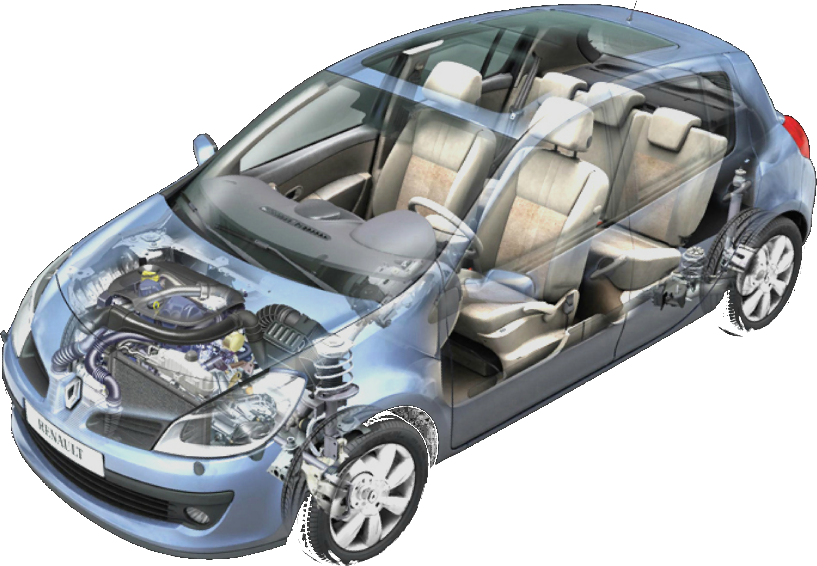
\includegraphics[width=4cm]{png/voiture} &&
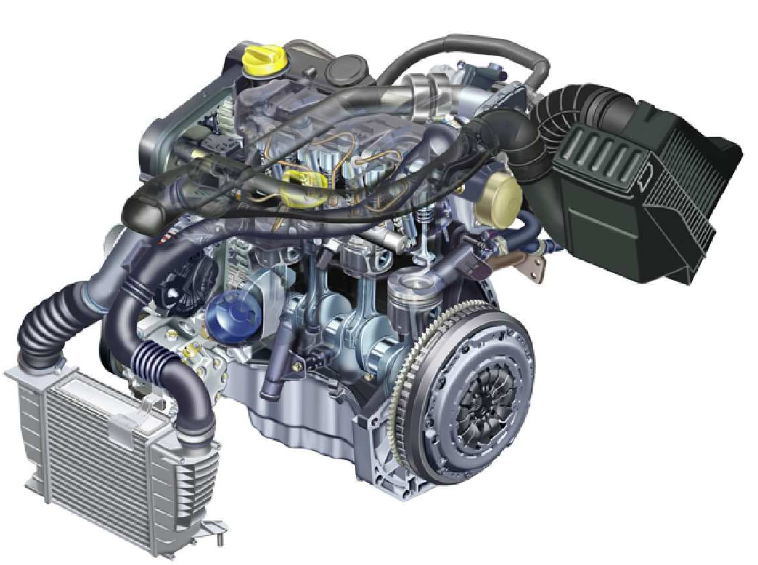
\includegraphics[height=4cm]{png/moteur} && 
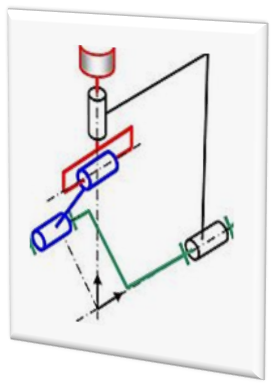
\includegraphics[height=4cm]{png/ex_schema}\\
\textit{Effeuillage d'un Renault Clio \cite{cite1}} &&
\textit{Moteur 1.5 dCi K9K 105 ch \cite{cite1}} &&
\textit{Modélisation par schéma cinématique\cite{cite2}}\\
\end{tabular}
\end{center}

\vspace{.2cm}
Les systèmes peuvent être constitués de 1 à plusieurs milliers de pièces, appelés encore solides. 
Ces solides sont liés les uns aux autres pour transmettre des efforts ou des mouvements. La cinématique permet d'étudier les mouvements relatifs entre les solides.

Nous nous intéresserons principalement à des systèmes existants. La géométrie des solides ne permettant pas toujours une étude aisée, nous commencerons par introduire des outils permettant de modéliser ces systèmes. 

\begin{prob}
\textsc{Problématique :}
\begin{itemize}
\item Quels sont les mouvements relatifs existants entre les solides qui constituent un mécanisme ?
\item Quels sont les outils graphiques pour modéliser ces mécanismes ?
\end{itemize}
\end{prob}

\begin{savoir}
\textsc{Savoirs :}
\begin{itemize}
\item Identifier la nature des contacts entre les solides.
\item Proposer une liaison cinématique associé au contact entre solides.
\item Réaliser un graphe de structure.
\item Réaliser un schéma cinématique (schéma cinématique minimal et schéma d'architecture).
\end{itemize}
\end{savoir}

\begin{rem}
Le but de ce cours est de présenter des méthodes pour modéliser un système mécanique par un schéma cinématique. Suivant les points de vues, d'autres méthodes peuvent être envisagées.

La complexité des contacts entre les solides est telle que les modèles choisis pour modéliser les liaisons peuvent faire l'objet de discussion. J'insiste donc sur le fait que les outils proposés \textbf{ne sont que des modèles} associés à des \textbf{objets réels}.
\end{rem}

\setlength{\parskip}{0ex plus 0.2ex minus 0ex}
 \renewcommand{\contentsname}{}
 \renewcommand{\baselinestretch}{1}

% \vspace{1cm}
\textit{Ce document est en évolution permanente. Merci de signaler toutes
erreurs ou coquilles.}

\tableofcontents

 \renewcommand{\baselinestretch}{1.2}
\setlength{\parskip}{2ex plus 0.5ex minus 0.2ex}






\section{Schéma technologique}
Une première étape pour modéliser un mécanisme peut être de passer par un schéma dit technologique. Ce type de schéma n'est pas normalisé. Il permet de représenter un système ainsi que certaines solutions technologiques qui sont utilisées. 

Lors de \textbf{l'analyse d'un mécanisme} ce schéma permet de disséquer un plan ou un système pour comprendre son fonctionnement. 

En phase de \textbf{conception d'un mécanisme} ce schéma est utilisé pour proposer des choix de solutions techniques. 

\subsection{Classes d'équivalence cinématique}

\begin{defi}
Une classe d'équivalence cinématique est un ensemble de pièces en liaison encastrement (démontable ou non). Toutes les pièces faisant partie d'une même classe d'équivalence n'ont pas de mobilités relatives entre elles. Elles ont le même mouvement lors du fonctionnement du mécanisme.
\end{defi}

Lorsqu'on veut établir un schéma cinématique, la première étape est de définir les différentes classes d'équivalence. 

\begin{methode}
On commence usuellement par repérer le bâti que l'on colorie, de préférence, avec une couleur claire. On identifie alors l'ensemble de pièces reliées au bâti par l'intermédiaire de vis ou d'autres éléments filetés.

On cherche alors à identifier une pièce qui semble importante lors de l'utilisation d'un mécanisme (un arbre par exemple). De même que précédemment, on recherche l'ensemble des pièces liées à cette dernière.

On répertorie ensuite (par exemple dans un tableau) les pièces appartenant aux différentes classes d'équivalence.
\end{methode}

\begin{rem}
\begin{minipage}[c]{.6\linewidth}
Les pièces qui sont en liaison encastrement démontables ne sont pas toujours assemblées par des vis. En effet, des pièces peuvent être serrées entre elles par l'intermédiaire d'un ajustement. 
Nous verrons plus tard comment indiquer sur un dessin quel est la nature de l'ajustement entre 2 pièces. Elles peuvent aussi être soudées.

Ici rien n'indique que l'axe est encastré dans le piston ou dans la bielle. 

On peut aussi s'aider de la nomenclature et du nom des pièces, dans les cas litigieux, pour classer les pièces dans des CEC.
\end{minipage} \hfill
\begin{minipage}[c]{.3\linewidth}
\begin{center}
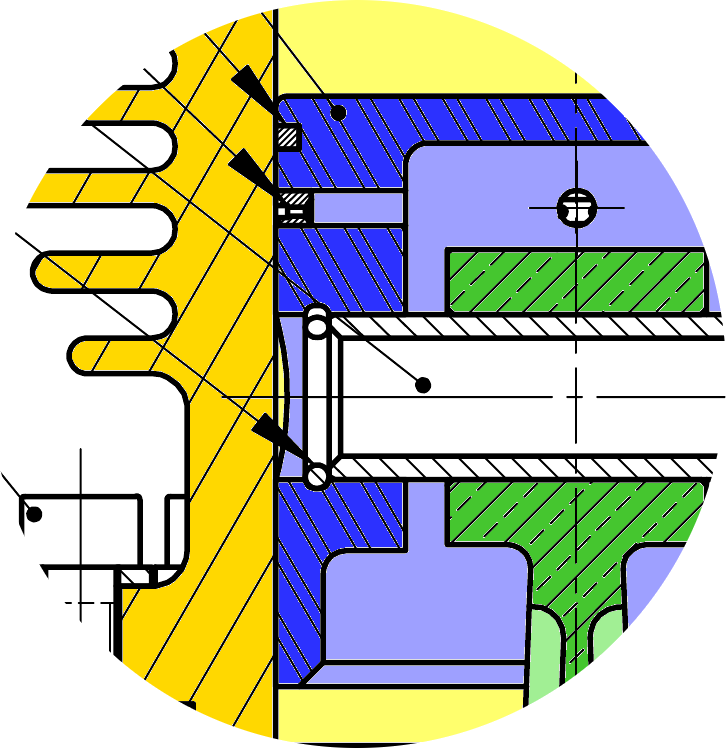
\includegraphics[width=.9\textwidth]{png/axe}
\end{center}
\end{minipage}
\end{rem}

\begin{exemple}
Dans le cas du micro compresseur, colorier chacune des classes d'équivalence avec une couleur différente.
\end{exemple}

\ifthenelse{\boolean{prof}}{%
\begin{center}
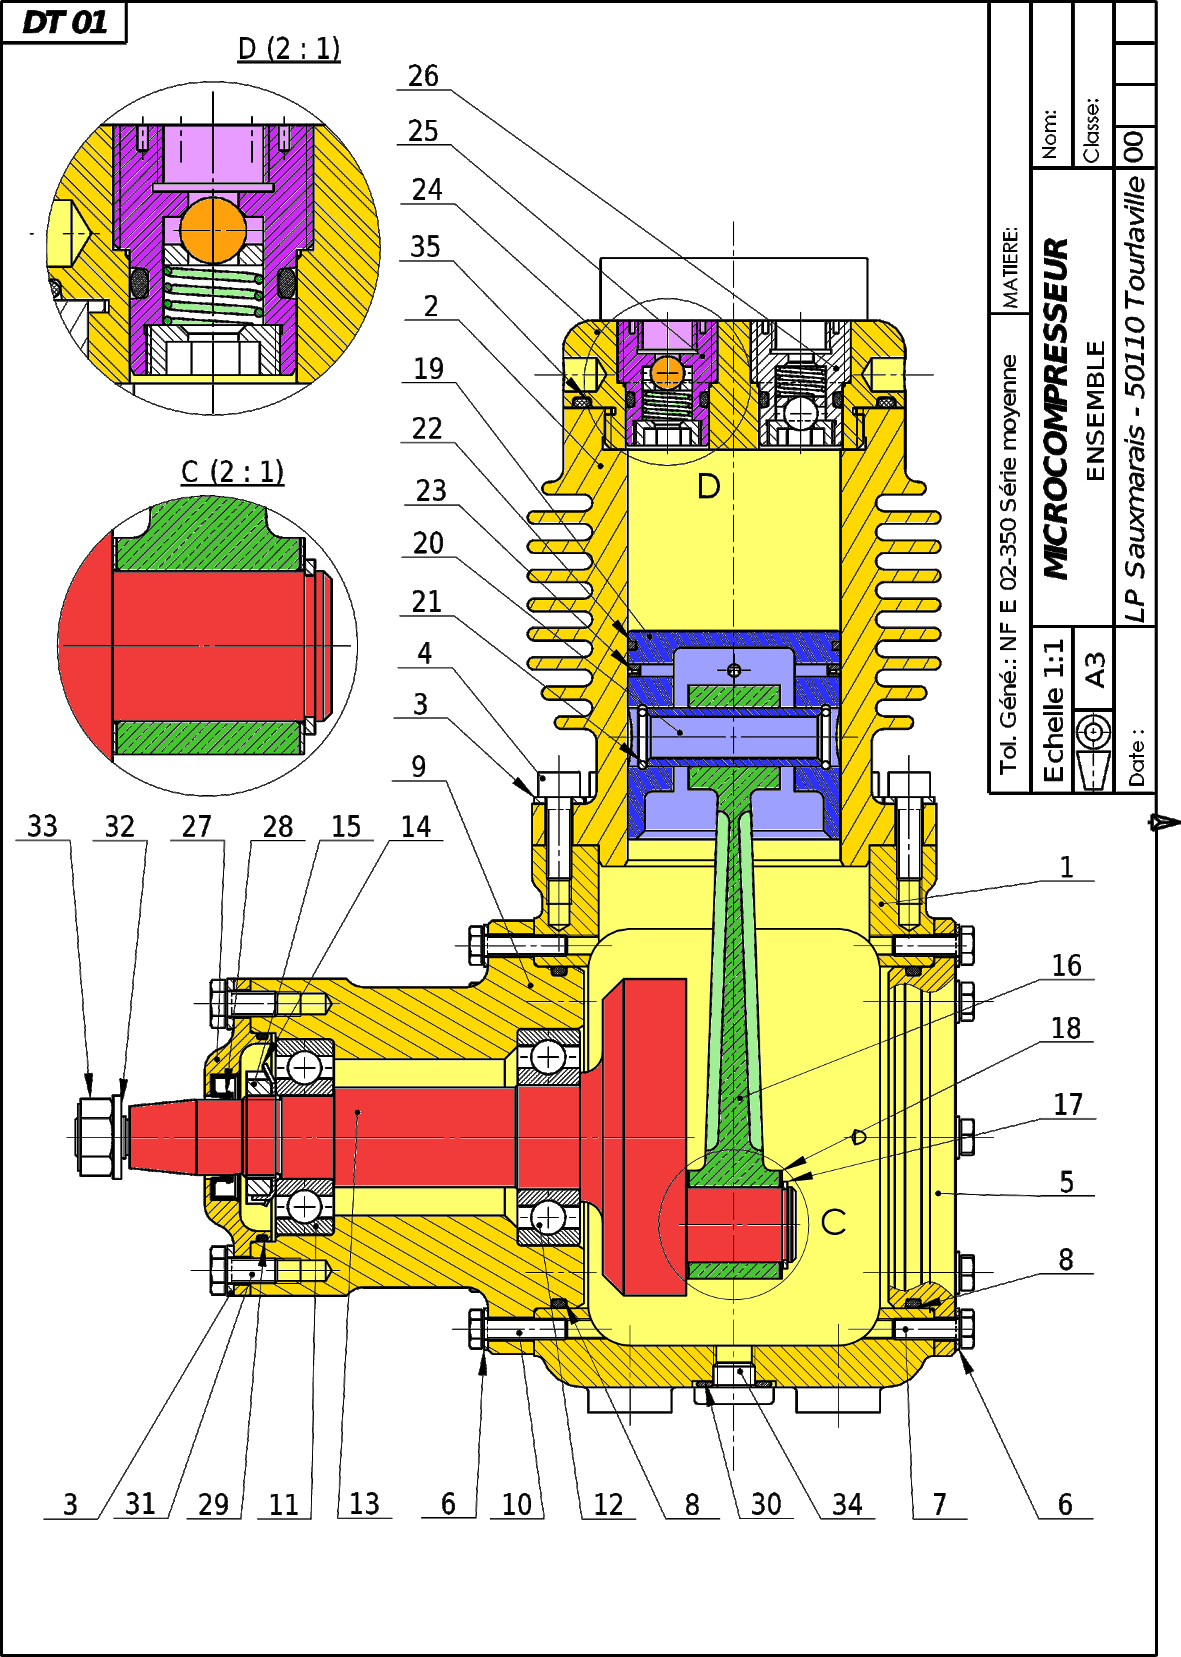
\includegraphics[width=.9\textwidth]{png/micro_cec}
\end{center}
}{%
}


\begin{exemple}
Identifier les classes d'équivalence cinématique. 
\ifthenelse{\boolean{prof}}{%

\begin{center}
\begin{tabular}{|p{3cm}|p{11cm}|}
\hline
& \\
Classe d'équivalence & Pièces \\
& \\
\hline
& \\
A & 1, 2, 3, 4, 5, 6, 7, 8, 9, 10, 24, 27, 28, 29, 30, 31, 34, 35 (25, 26) \\
& \\
\hline
& \\
B & 19, 20, 21, 22, 23  \\
& \\
\hline
& \\
C & 16\\
& \\
\hline
& \\
D & 13, 14, 15, 17, 18, 32, 33\\
& \\
\hline
\end{tabular}
\end{center}
}{%
}
\end{exemple}

\subsection{Schéma technologique}

\begin{defi}

Le schéma technologique n'est pas un schéma normalisé. Les différentes pièces sont représentées sous forme filaire. Les contacts entre les pièces sont représentés. Les composants technologiques sont représentés sous forme schématique. 

\end{defi}


\begin{exemple}
Représentation entre la boîte à roulements 9 et la boîte à joint 27.

Le schéma technologique met en avant les zones de contacts entre ces 2 pièces : on y fait apparaître clairement la zone de contact plane ainsi que la "petite" zone cylindrique. Ce contact cylindre cylindre est appelé \textbf{centrage court} (Le rapport entre la longueur de contact et le diamètre du cylindre est inférieur à 1.). 
\begin{center}
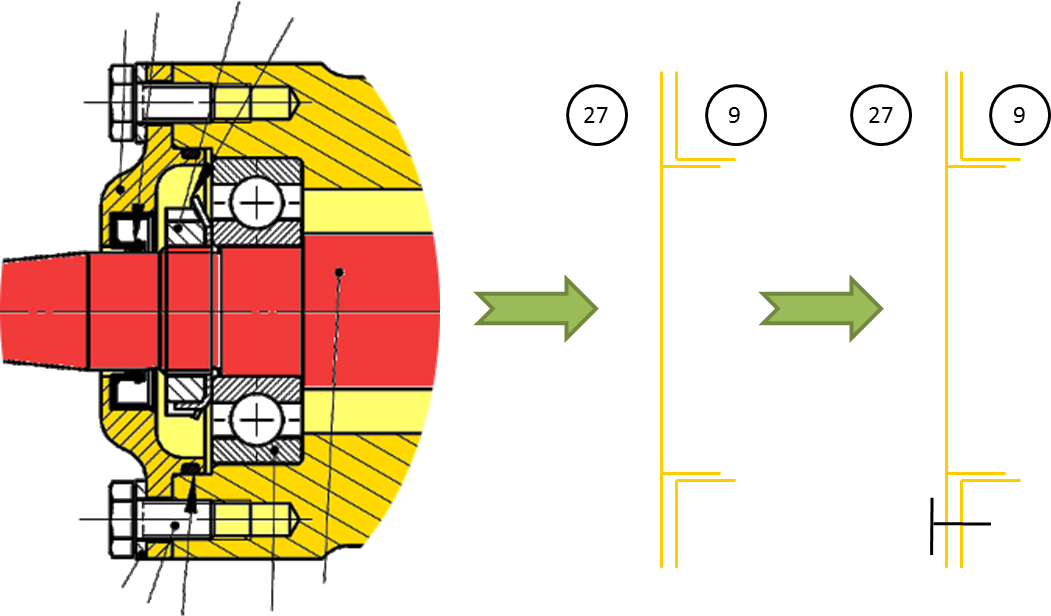
\includegraphics[width=.6\textwidth]{png/schema_1}
\end{center}
\end{exemple}

\begin{rem}
Il est possible, si cela n'a pas d'intérêt pour la modélisation, de ne pas représenter les contacts au sein d'une même classe d'équivalence.
\end{rem}

\subsection{Représentation d'éléments standards}
Pour dessiner les éléments standards de la construction mécanique comme les roulements ou les joints, il existe une représentation spécifique.

Les roulements permettent d'assurer un guidage en rotation entre deux éléments.

\begin{minipage}[c]{.35\linewidth}
\begin{center}
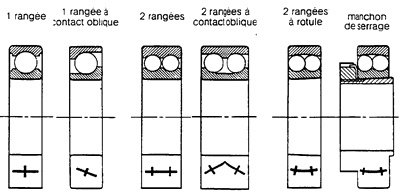
\includegraphics[width=.95\textwidth]{png/roulements1}
\end{center}
\end{minipage}\hfill
\begin{minipage}[c]{.35\linewidth}
\begin{center}
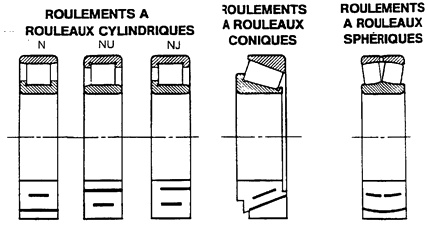
\includegraphics[width=.95\textwidth]{png/roulements2}
\end{center}
\end{minipage}\hfill
\begin{minipage}[c]{.2\linewidth}
\begin{center}
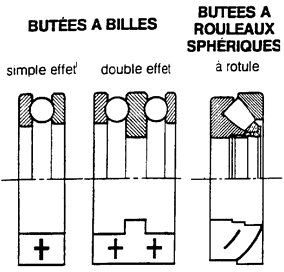
\includegraphics[width=.95\textwidth]{png/roulements3}
\end{center}
\end{minipage}


Les joints présentés ci-dessous \cite{gdi} assurent une étanchéité dynamique entre deux pièces en mouvement relatif. 
\begin{minipage}[c]{.45\linewidth}
\begin{center}
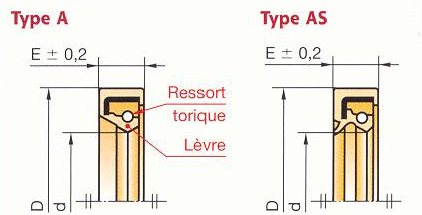
\includegraphics[width=.95\textwidth]{png/joint_1}

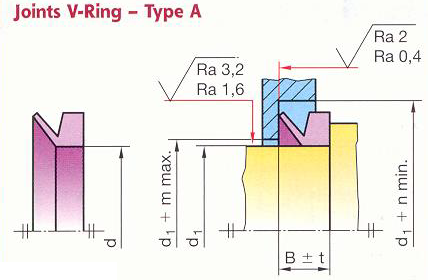
\includegraphics[width=.95\textwidth]{png/joint_2}
\end{center}
\end{minipage}\hfill
\begin{minipage}[c]{.45\linewidth}
\begin{center}
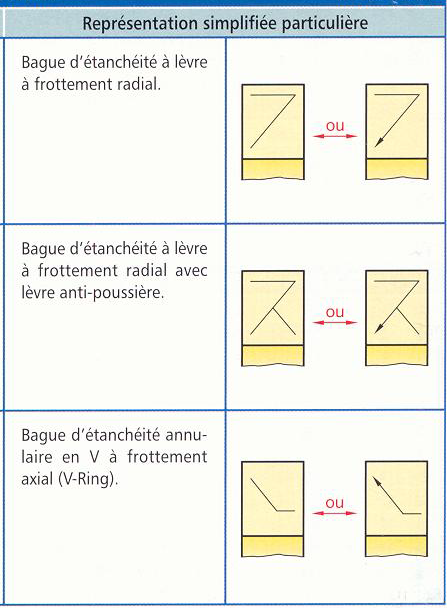
\includegraphics[width=.95\textwidth]{png/joint_3}
\end{center}
\end{minipage}

\subsection{Exemple}

\begin{exemple}
Réaliser le schéma technologique associé au compresseur.
\end{exemple}

\ifthenelse{\boolean{prof}}{%
\begin{minipage}[b]{.45\linewidth}
\begin{center}
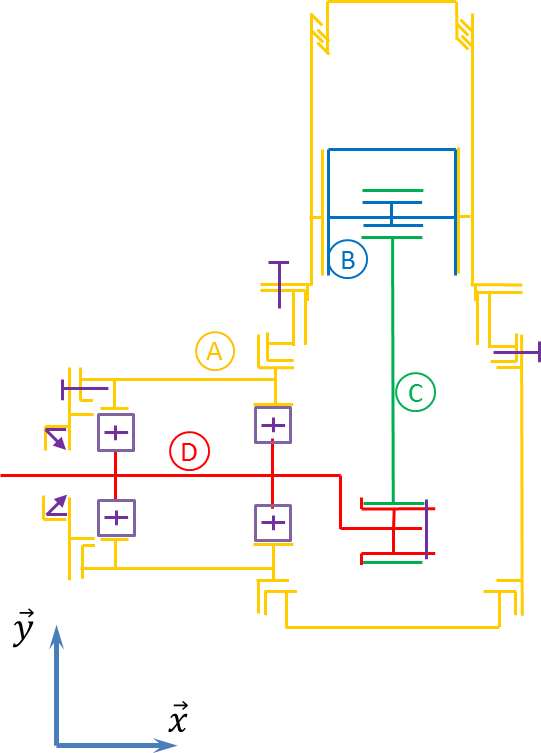
\includegraphics[width=.95\textwidth]{png/techno_1}

\textit{Détail du carter}
\end{center}
\end{minipage}\hfill
\begin{minipage}[b]{.45\linewidth}
\begin{center}
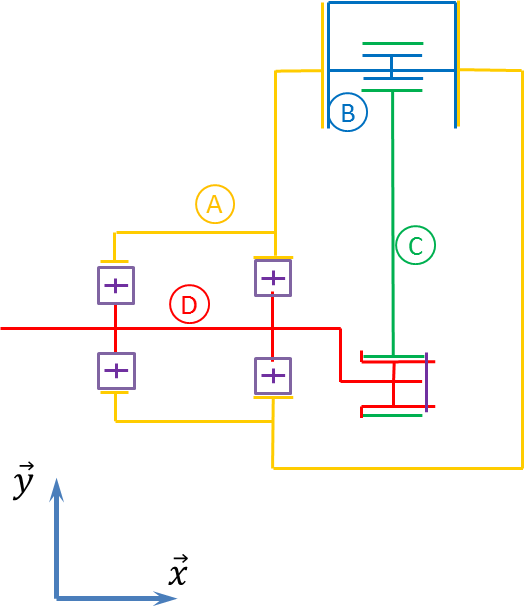
\includegraphics[width=.95\textwidth]{png/techno_2}

\textit{Carter simplifié}
\end{center}
\end{minipage}
}{%
}

\ifthenelse{\boolean{prof}}{%
}{%
}

\begin{rem}
On peut dès lors indiquer un repère orthonormé sur le schéma. 
\end{rem}
\section{Modélisation des contacts entre solide}

\subsection{Le graphe de structure}
\begin{defi}
Le graphe de structure permet d'avoir une vue d'ensemble sur un mécanisme. Dans ce graphe :
\begin{itemize}
\item les classes d'équivalence sont représentées par des cercles;
\item les liaisons (ou contacts) entre les classes sont représentées par des arc.
\end{itemize} 
On définit 3 types de chaînes :
\begin{center}
\begin{tabular}{ccc}
Les chaînes ouvertes & Les chaînes fermées & Les chaînes complexes \\
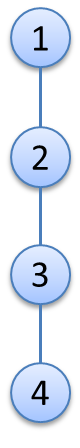
\includegraphics[height=3cm]{png/co.png}
&
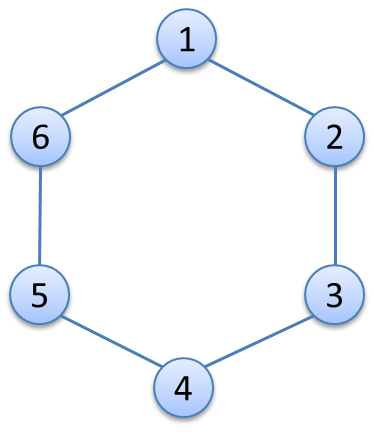
\includegraphics[height=3cm]{png/cf.png}
&
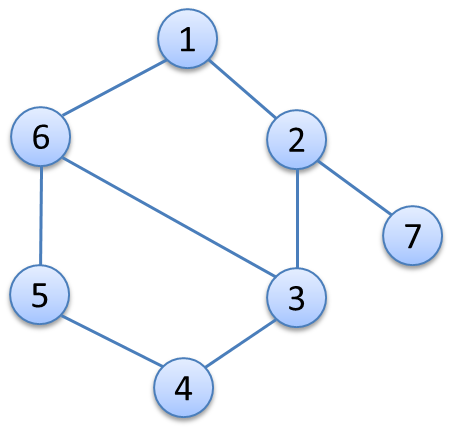
\includegraphics[height=3cm]{png/cc.png}\\
\end{tabular}
\end{center}


\begin{center}
\begin{tabular}{ccc}
Liaisons en serie & & Liaisons en parallèle\\
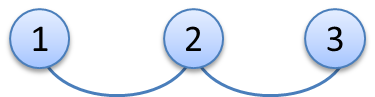
\includegraphics[height=1.5cm]{png/serie.png}
&
%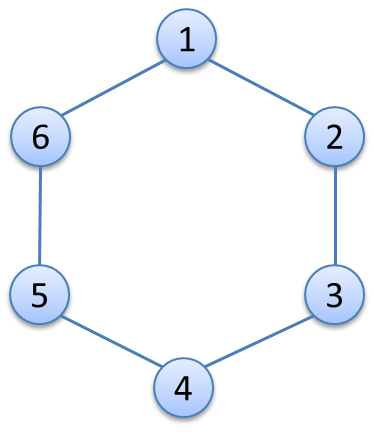
\includegraphics[height=3cm]{png/cf.png}
&
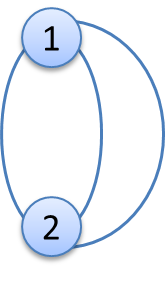
\includegraphics[height=4cm]{png/parallele.png}\\
\end{tabular}
\end{center}
\end{defi}

\begin{rem}
\textbf{Tous} les contacts \textbf{permanents} sont à représenter dans ce graphe.

Les contacts qui peuvent se désolidariser pendant le fonctionnement ou à cause des jeux ne sont pas à prendre en compte. 

\textbf{Dès lors, les pièces déformables (les ressorts par exemple) ne seront plus représentés.}
\end{rem}

\begin{exemple}
Réaliser le graphe de structure du compresseur.
\ifthenelse{\boolean{prof}}{%
\begin{center}
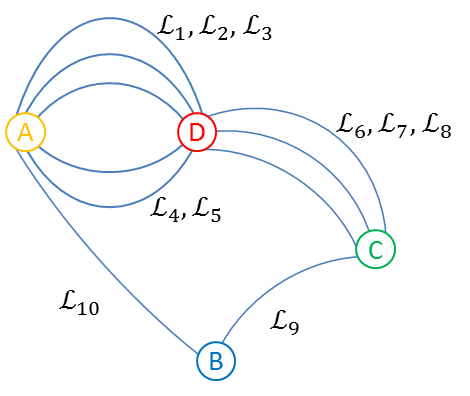
\includegraphics[width=.4\textwidth]{png/graphe}
\end{center}
}{%
}
\end{exemple}

\subsection{Identification des liaisons entre solides ou entre CEC}

\subsubsection{Surfaces de contact}

\begin{defi}
Les surfaces de contact désignent les entités géométriques qui sont en contact entre deux solides ou deux classes d'équivalence. Elles correspondent à chaque liaison citée dans le graphe de structure.

Elles sont toujours associées par paire. Une surface élémentaire peut être de type sphérique, cylindrique, plane...
\end{defi}

\begin{rem}
\begin{minipage}[c]{.7\linewidth}
\textbf{Dimension de la zone de contact :} on veillera à bien visualiser les dimensions de la zone de contact. 

Par exemple, dans le cas des cylindres, on veillera à déterminer le rapport entre la longueur de guidage et le diamètre.
\end{minipage}
\hfill
\begin{minipage}[c]{.25\linewidth}
\begin{center}
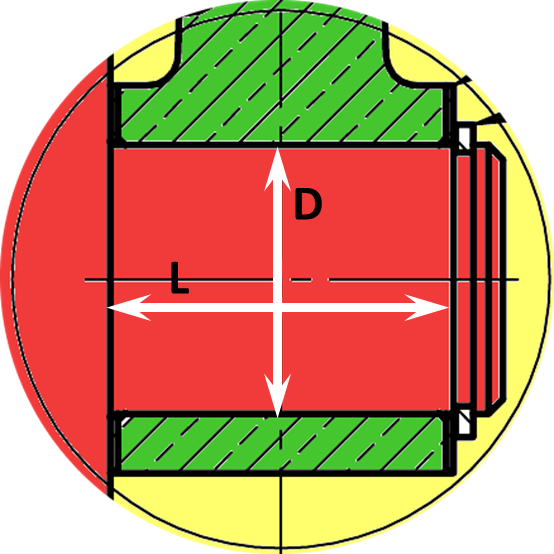
\includegraphics[width=.9\textwidth]{png/rapportLD}
\end{center}
\end{minipage}
\end{rem}

\begin{exemple}
Donner la nature des surfaces pour chacune des liaisons du compresseur. 

\ifthenelse{\boolean{prof}}{%
\begin{itemize}
\item $\mathcal{L}_1$ : contact cylindre -- cylindre;
\item $\mathcal{L}_2$ : contact cylindre -- cylindre;
\item $\mathcal{L}_3$ : contact cylindre -- cylindre;
\item $\mathcal{L}_4$ : contact plan -- plan;
\item $\mathcal{L}_5$ : contact plan -- plan;
\item $\mathcal{L}_6$ : contact cylindre -- cylindre;
\item $\mathcal{L}_7$ : contact plan -- plan;
\item $\mathcal{L}_8$ : contact cylindre -- cylindre;
\item $\mathcal{L}_9$ : contact plan -- plan.
\end{itemize}

}{%
}
\end{exemple}



\subsection{Notion de degrés de liberté et de degrés de liaison}
\begin{defi}
\textbf{Degrés de liberté}

On considère un solide $S_1$ en mouvement par rapport à un solide $S_0$. Le mouvement entre les deux solides peut, au maximum, se décomposer en 6 mouvements élémentaires appelés 6 degrés de liberté:

\vspace{.25cm}

\begin{minipage}[c]{.44\linewidth}
\begin{itemize}
\item une translation $T_x$ suivant la direction $\overrightarrow{x_0}$;
\item une translation $T_y$ suivant la direction $\overrightarrow{y_0}$;
\item une translation $T_z$ suivant la direction $\overrightarrow{z_0}$;
\end{itemize}
\end{minipage} \hfill
\begin{minipage}[c]{.55\linewidth}
\begin{itemize}
\item une rotation $R_x$ autour d'un axe parallèle à $\left(0,\overrightarrow{x_0}\right)$;
\item une rotation $R_y$ autour d'un axe parallèle à $\left(0,\overrightarrow{y_0}\right)$;
\item une rotation $R_z$ autour d'un axe parallèle à $\left(0,\overrightarrow{z_0}\right)$.
\end{itemize}
\end{minipage}
\end{defi}

\begin{exemple}

\begin{minipage}[c]{.46\linewidth}
Lorsqu'un avion se déplace dans le ciel, il peut se déplacer suivant les 6 degrés de liberté. Ces 6 mouvements portent alors des noms particuliers : 
\begin{itemize}
\item $T_x$ est appelée l'avancement;
\item $T_y$ est appelée la dérive;
\item $T_z$ est appelée l'ascension ou la descente;
\item $R_x$ est appelée le roulis;
\item $R_y$ est appelée le tangage;
\item $R_z$ est appelée le lacet.
\end{itemize}
\end{minipage}\hfill
\begin{minipage}[c]{.46\linewidth}
\begin{center}
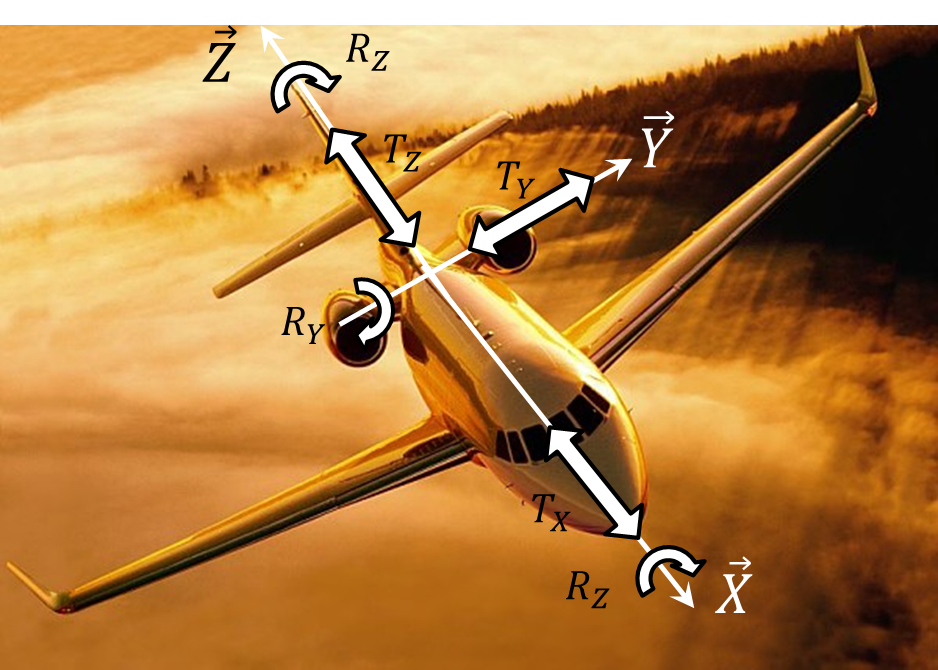
\includegraphics[width=.9\textwidth]{png/avion}

\textit{Falcon 2000 -- Dassault Aviation \cite{cite6}}
\end{center}
\end{minipage}

\vspace{.25cm}

\begin{center}
\begin{tabular}{ccc}
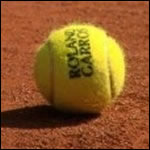
\includegraphics[height=2cm]{png/balle} 
& 
\includegraphics[height=2cm]{png/tube} 
& 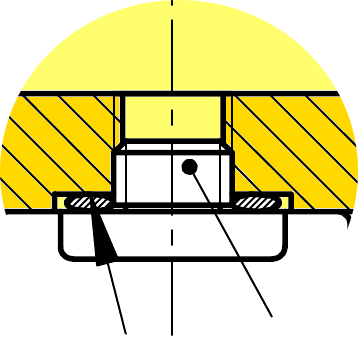
\includegraphics[height=2cm]{png/vis} 
\end{tabular}
\end{center}


\begin{center}
\begin{tabular}{|l|c|c|c|c|c|c|}

\hline 
Mouvements & $T_x$ & $T_y$ & $T_z$ &  $R_x$ &  $R_y$ &  $Y_z$ \\
\hline 
Mouvement d'une balle par rapport le sol & & & & & & \\
\hline 
Mouvement d'une balle de tennis par rapport à un tube & & & & & & \\
\hline 
Mouvement du tube par rapport à une table lorsqu'il est posé sur le coté  & & & & & & \\
\hline 
Mouvement du tube par rapport à une table lorsqu'il est posé à plat  & & & & & & \\
\hline 
Mouvement d'une vis par rapport à un écrou  & & & & & & \\
\hline 
Mouvement d'une roue de vélo par rapport au cadre  & & & & & & \\
\hline 
Mouvement ... & & & & & & \\
\hline 
\end{tabular}
\end{center}

\end{exemple}


\begin{defi}
\textbf{Degrés de liaisons}

On considère un solide $S_1$ fixe par rapport à un solide $S_0$. Les efforts transmissibles  entre les deux solides peuvent, au maximum, se décomposer en 6 efforts élémentaires appelés 6 degrés de liaisons:
\vspace{.25cm}

\begin{minipage}[c]{.4\linewidth}
\begin{itemize}
\item un effort transmissible $F_x$ suivant la direction $\overrightarrow{x_0}$;
\item un effort transmissible $F_y$ suivant la direction $\overrightarrow{y_0}$;
\item un effort transmissible $F_z$ suivant la direction $\overrightarrow{z_0}$;
\end{itemize}
\end{minipage} \hfill
\begin{minipage}[c]{.4\linewidth}
\begin{itemize}
\item un couple transmissible $C_x$ autour d'un axe parallèle à $\left(0,\overrightarrow{x_0}\right)$;
\item un couple transmissible $C_y$autour d'un axe parallèle à $\left(0,\overrightarrow{y_0}\right)$;
\item un couple transmissible $C_z$autour d'un axe parallèle à $\left(0,\overrightarrow{z_0}\right)$.
\end{itemize}
\end{minipage}

\vspace{.25cm}

Un effort s'exprime en Newton ($N$) et un couple en Newton - mètres ($N\cdot m$).
\end{defi}

\begin{exemple}
\begin{center}
\begin{tabular}{|l|c|c|c|c|c|c|}

\hline 
Effort & $F_x$ & $F_y$ & $F_z$ &  $C_x$ &  $C_y$ &  $C_z$ \\
\hline 
Effort d'une balle sur le sol & & & & & & \\
\hline 
Effort d'une balle de tennis dans un tube & & & & & & \\
\hline 
Effort du tube sur une table lorsqu'il est posé sur le coté  & & & & & & \\
\hline 
Effort du tube sur une table lorsqu'il est posé à plat  & & & & & & \\
\hline 
Effort d'une vis sur un écrou  & & & & & & \\
\hline 
Effort d'une roue de vélo sur le cadre  & & & & & & \\
\hline 
Effort ... & & & & & & \\
\hline 
\end{tabular}
\end{center}


\end{exemple}


\begin{resultat}
Lorsque deux solides sont liés, on a : 
\begin{center}
degré de liberté + degré de liaison = 6
\end{center}
\end{resultat}






\newpage

\subsection{Modélisation des liaisons cinématiques}
\subsubsection{Hypothèse}
Lors de la modélisation des liaisons cinématiques, différentes hypothèses pourront être faites :
\begin{itemize}
\item les surfaces peuvent être considérées comme parfaites; 
\item les liaisons peuvent être considérées sans jeu.
\end{itemize}

Attention, en TP, il faudra vérifié si ces hypothèses sont applicables ou non.

\subsubsection{Liaison encastrement}
La liaison encastrement est une liaison où il y a aucun degré de liberté. 

La liaison encastrement peut être réalisée par association de plusieurs solides (voir cours sur la conception des liaisons encastrement démontables) ou par soudage (voir cours sur le soudage).


\subsubsection{Liaison glissière}


\begin{center}
\begin{tabular}{p{.45\textwidth} c p{.45\textwidth}}
\hline
& &\\
Définition et hypothèses : 

une liaison glissière d'axe $\vect{x_1}$ entre $S_1$ et $S_2$ autorise une translation d'axe $\vect{x_1}$ entre $S_1$ et $S_2$. 
&& Nature des surfaces en contact :
\begin{center}
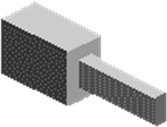
\includegraphics[height=2cm]{png/glissiere_S1}
\hspace{.5cm}
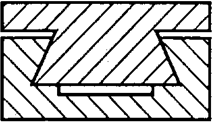
\includegraphics[height=2cm]{png/glissiere_S2}
\end{center}
\\
&& \\
\hline
&& \\
Degrés de liberté : $T_X$
&& Degrés de liaison : $F_Y$, $F_Z$, $C_X$, $C_Y$, $C_Z$. \\
&& \\
\hline
\begin{center}
\textit{Symbole 3d}

\includegraphics[height=3cm]{png/glissiere_3d} 
\end{center}

&&
\begin{center}
\textit{Symbole 2d}

\includegraphics[height=3cm]{png/glissiere_2d} 
\end{center}\\
\hline
\multicolumn{3}{c}{\textit{Paramétrage}}\\
\begin{center}
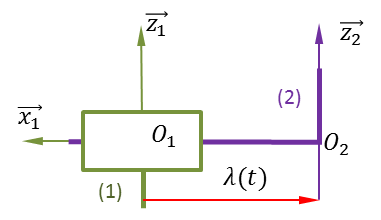
\includegraphics[height=3cm]{png/glissiere_p} 
\end{center}& &
Il faut paramétrer la translation $T_X$ :

$\vect{O_1O_2}(t)=\lambda(t) \vect{x_1}$
\\
\hline 
&&
\begin{center}
\textit{Douille à billes}

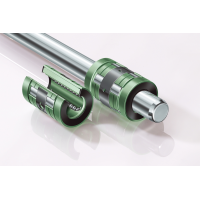
\includegraphics[height=3cm]{png/douille} 
\end{center}\\
\hline 
\end{tabular}
\end{center}

\newpage

\subsubsection{Liaison pivot}
\begin{center}
\begin{tabular}{p{.45\textwidth} c p{.45\textwidth}}
\hline
& &\\
Définition et hypothèses : 

une liaison pivot d'axe $\vect{x_1}$ entre $S_1$ et $S_2$ autorise une rotation d'axe $\vect{x_1}$ entre $S_1$ et $S_2$. 
&& Nature des surfaces en contact :

Surfaces de révolutions \textbf{sauf les cylindres}. Le rapport $L/D$ doit être supérieur à 1,5.

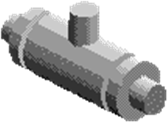
\includegraphics[height=2cm]{png/pivot_s.png} 
\\
&& \\
\hline
&& \\
Degrés de liberté : $R_X$
&& Degrés de liaison : $F_X$, $F_Y$, $F_Z$, $C_Y$, $C_Z$. \\
&& \\
\hline
\multicolumn{3}{p{.9\textwidth}}{
\begin{center}
\begin{tabular}{cc}
\textit{Symbole 3d} & \textit{Symbole 2d} \\
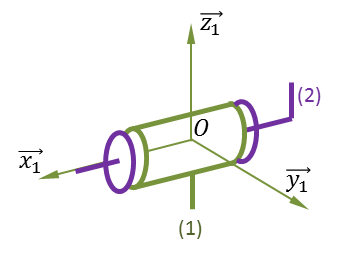
\includegraphics[height=3cm]{png/pivot_3d} 
&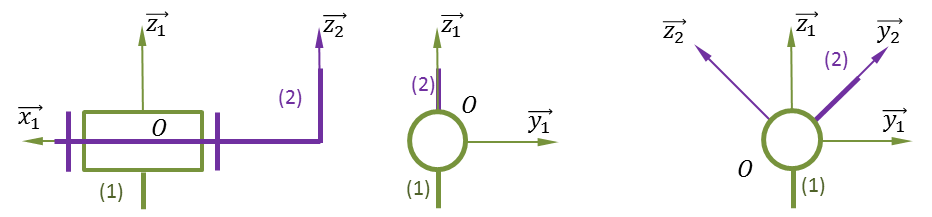
\includegraphics[height=3cm]{png/pivot_2d} \\
\end{tabular}
\end{center}
}\\
\hline
\multicolumn{3}{c}{\textit{Paramétrage}}\\
\begin{center}
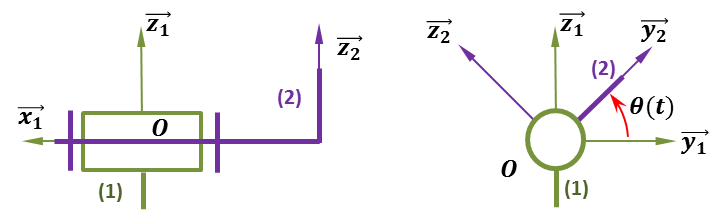
\includegraphics[height=3cm]{png/pivot_p} 
\end{center}& &
Il faut paramétrer la rotation $R_X$ :

%$\vect{O_1O_2}(t)=\lambda(t) \vect{x_1}$
\\
\hline 
\begin{center}
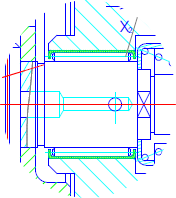
\includegraphics[height=3cm]{png/ex_pivot} 
\end{center}
&&
\begin{center}
\textit{Roulement à aiguilles}

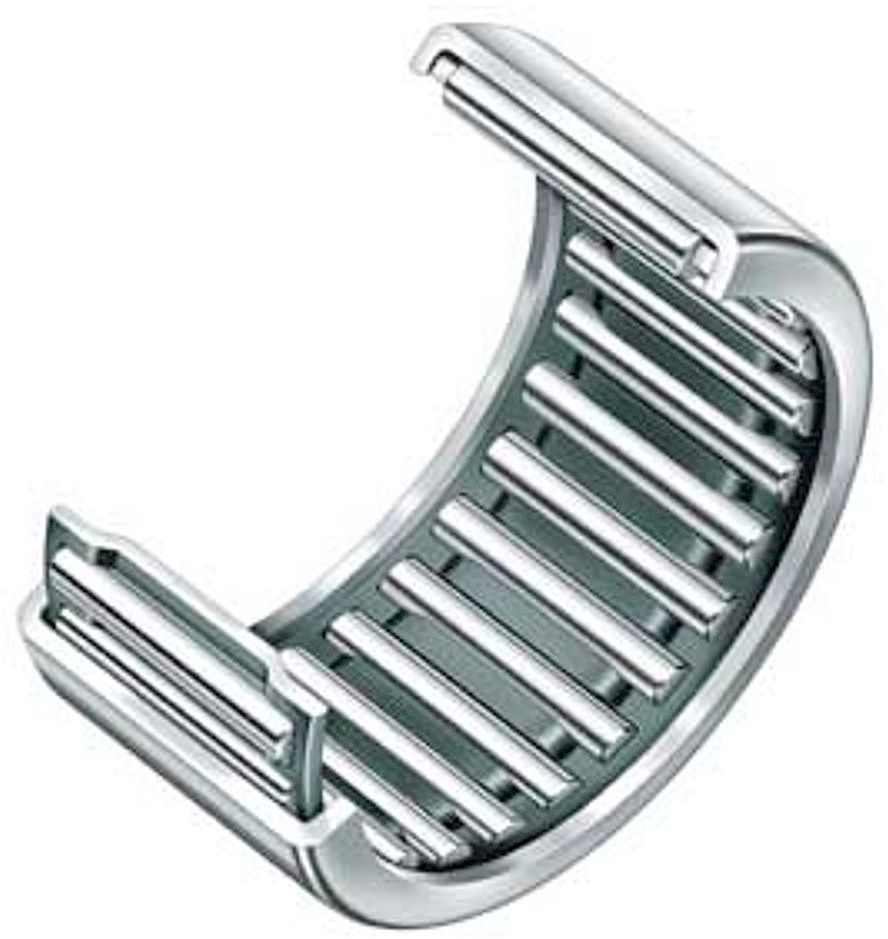
\includegraphics[height=3cm]{png/aiguille} 
\end{center}\\
\hline 
\end{tabular}
\end{center}

\subsubsection{Liaison glissière hélicoïdale}
\begin{center}
\begin{tabular}{p{.45\textwidth} c p{.45\textwidth}}
\hline
& &\\
Définition et hypothèses : 

une liaison glissière hélicoïdale d'axe $\vect{x_1}$ entre $S_1$ et $S_2$ autorise une rotation et une translation d'axe $\vect{x_1}$ entre $S_1$ et $S_2$. Ces deux mouvements sont liés par \textbf{le pas}.
&& Nature des surfaces en contact
 
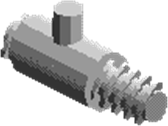
\includegraphics[height=2cm]{png/helico_s} \\
&& \\
\hline
&& \\
Degrés de liberté : $R_X$ et $T_X$
&& Degrés de liaison : $F_X$, $F_Y$, $F_Z$, $C_X$, $C_Y$, $C_Z$. \\
&& \\
\hline
\multicolumn{3}{p{.9\textwidth}}{
\begin{center}
\begin{tabular}{cc}
\textit{Symbole 3d} & \textit{Symbole 2d} \\
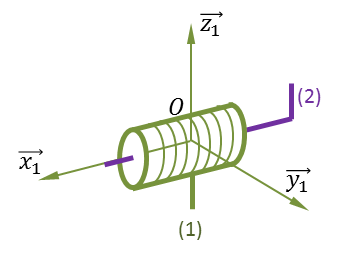
\includegraphics[height=3cm]{png/helico_3d} 
&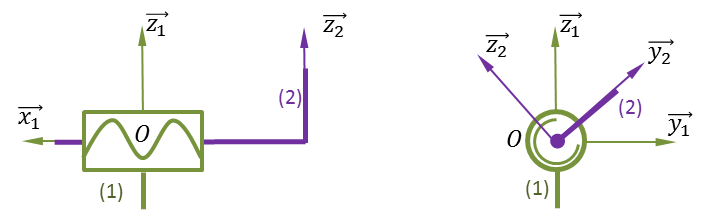
\includegraphics[height=3cm]{png/helico_2d} \\
\end{tabular}
\end{center}
}\\
\hline
\multicolumn{3}{c}{\textit{Paramétrage}}\\
\begin{center}
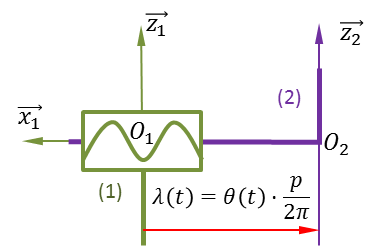
\includegraphics[height=3cm]{png/helico_p} 
\end{center}& &
Il faut paramétrer la translation $T_X$ et la rotation $R_X$. 


\\
\hline 
&&
\begin{center}
\textit{Vis à billles}

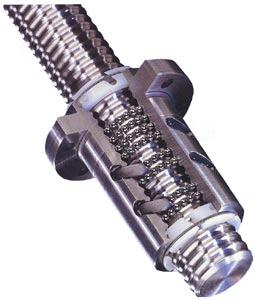
\includegraphics[height=3cm]{png/visbilles} 
\end{center}\\
\hline 
\end{tabular}
\end{center}

\subsubsection{Liaison pivot glissant}
\begin{center}
\begin{tabular}{p{.45\textwidth} c p{.45\textwidth}}
\hline
& &\\
Définition et hypothèses : 

une liaison pivot glissant d'axe $\vect{x_1}$ entre $S_1$ et $S_2$ autorise une rotation et une translation d'axe $\vect{x_1}$ entre $S_1$ et $S_2$. 
&& Nature des surfaces en contact :

Dans la plupart des cas, les surfaces de contact sont des cylindres dont $L/D>1,5$.

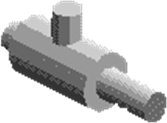
\includegraphics[height=2cm]{png/pivotg_s}
\\
&& \\
\hline
&& \\
Degrés de liberté : $R_X$ et $T_X$
&& Degrés de liaison : $F_Y$, $F_Z$, $C_Y$, $C_Z$. \\
&& \\
\hline
\multicolumn{3}{p{.9\textwidth}}{
\begin{center}
\begin{tabular}{cc}
\textit{Symbole 3d} & \textit{Symbole 2d} \\
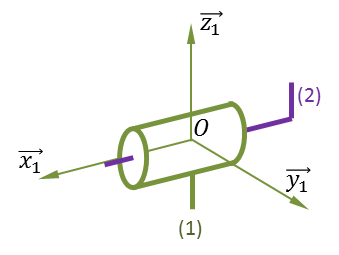
\includegraphics[height=3cm]{png/pivotg_3d} 
&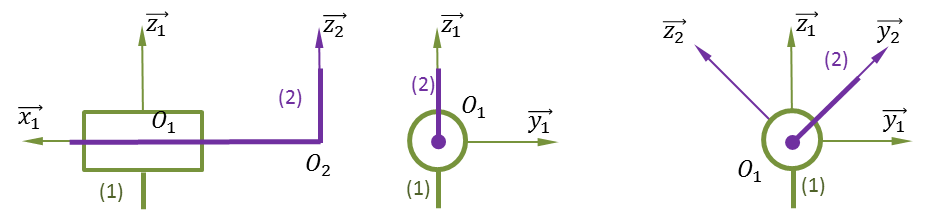
\includegraphics[height=3cm]{png/pivotg_2d} \\
\end{tabular}
\end{center}
}\\
\hline
\multicolumn{3}{c}{\textit{Paramétrage}}\\
\begin{center}
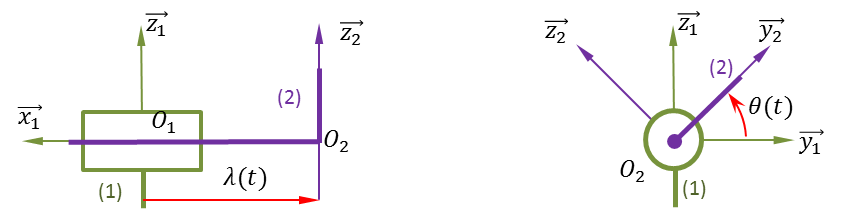
\includegraphics[height=3cm]{png/pivotg_p} 
\end{center}& &
Il faut paramétrer la translation $T_X$ et la rotation $R_X$. 


\\
\hline 
\begin{center}
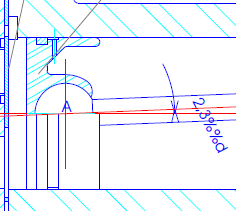
\includegraphics[height=3cm]{png/ex_pivotg} 
\end{center}
&&
\begin{center}
\textit{Coussinet en bronze}

\includegraphics[height=3cm]{png/coussinet} 
\end{center}\\
\hline 
\end{tabular}
\end{center}

\subsubsection{Liaison rotule à doigt}

\begin{center}
\begin{tabular}{p{.45\textwidth} c p{.45\textwidth}}
\hline
& &\\
Définition et hypothèses : 

une liaison rotule à doigt autorise deux rotations entre $S_1$ et $S_2$. 
&& Nature des surfaces en contact 

\includegraphics[height=2cm]{png/doigt_s} 
\\
&& \\
\hline
&& \\
Degrés de liberté : $R_X$ et $R_Y$
&& Degrés de liaison : $F_X$, $F_Y$, $F_Z$, $C_Z$. \\
&& \\
\hline
\multicolumn{3}{p{.9\textwidth}}{
\begin{center}
\begin{tabular}{cc}
\textit{Symbole 3d} & \textit{Symbole 2d} \\
\includegraphics[height=3cm]{png/doigt_3d} 
&\includegraphics[height=3cm]{png/doigt_2d} \\
\end{tabular}
\end{center}
}\\
\hline
\multicolumn{3}{c}{\textit{Paramétrage}}\\
\begin{center}
%\includegraphics[height=3cm]{png/doigt_p} 
\end{center}& &
Il faut paramétrer les rotations $R_X$ et $R_Y$. 
\vspace{3cm}

$\quad$

\\
\hline 
\end{tabular}
\end{center}


\subsubsection{Liaison appui plan}
\begin{center}
\begin{tabular}{p{.45\textwidth} c p{.45\textwidth}}
\hline
& &\\
Définition et hypothèses : 

une liaison appui plan de normale $\vect{z_1}$ entre $S_1$ et $S_2$ autorise une rotation autour de $\vect{z_1}$ et deux translations suivant $\vect{x_1}$ et $\vect{y_1}$ entre $S_1$ et $S_2$. 
&& Nature des surfaces en contact 

On note $L$ et $l$ les dimensions de la zone de contact. Dans le cas d'un appui plan, $L/l\simeq 1$. $L$ et $l$ sont du même ordre de grandeur que les dimensions du plus petit solide.

\includegraphics[height=2cm]{png/plan_s} 
\\

&& \\
\hline
&& \\
Degrés de liberté : $R_Z$, $T_X$  et $T_Y$
&& Degrés de liaison : $F_Z$, $C_X$, $C_Y$. \\
&& \\
\hline
\multicolumn{3}{p{.9\textwidth}}{
\begin{center}
\begin{tabular}{cc}
\textit{Symbole 3d} & \textit{Symbole 2d} \\
\includegraphics[height=3cm]{png/plan_3d} 
&\includegraphics[height=3cm]{png/plan_2d} \\
\end{tabular}
\end{center}
}\\
\hline
\multicolumn{3}{c}{\textit{Paramétrage}}\\
\begin{center}
\includegraphics[height=3cm]{png/plan_p} 
\end{center}& &
Il faut paramétrer les translation $T_X$ et $T_Y$ et la rotation $R_Z$. 


\\
\hline
\begin{center}
\rotatebox{90}{\includegraphics[width=1.5cm]{png/ex_plan}}
\end{center}
&&
\begin{center}
\textit{Butée à aiguilles}

\includegraphics[height=3cm]{png/butee} 
\end{center}\\
\hline 
\end{tabular}
\end{center}


\subsubsection{Liaison rotule}
\begin{center}
\begin{tabular}{p{.45\textwidth} c p{.45\textwidth}}
\hline
& &\\
Définition et hypothèses : 

une liaison rotule entre $S_1$ et $S_2$ autorise trois rotations. 
&& Nature des surfaces en contact :

Les surfaces en contact peuvent être des cercles, des sphères ou des "cylindres courts". Dans ce cas, $L/D << 0,5$

\includegraphics[height=2cm]{png/rotule_s} 
\\
&& \\
\hline
&& \\
Degrés de liberté : $R_X$, $R_Y$ et $R_Z$
&& Degrés de liaison : $F_X$, $F_Y$, $F_Z$. \\
&& \\
\hline
\multicolumn{3}{p{.9\textwidth}}{
\begin{center}
\begin{tabular}{cc}
\textit{Symbole 3d} & \textit{Symbole 2d} \\
\includegraphics[height=3cm]{png/rotule_3d} 
&\includegraphics[height=3cm]{png/rotule_2d} \\
\end{tabular}
\end{center}
}\\
\hline
\multicolumn{3}{c}{\textit{Paramétrage}}\\
\begin{center}
%\includegraphics[height=3cm]{png/rotule_p} 
\end{center}

\vspace{3cm}

$\quad$
& &
Il faut paramétrer les rotations $R_X$, $R_Y$ et $R_Z$. 


\\
\hline 
\begin{center}
\includegraphics[height=3cm]{png/ex_rotule} 
\end{center}
&&
\begin{center}
\textit{Roulement à rotule sur billes}

\includegraphics[height=3cm]{png/rltrotule.png} 
\end{center}\\
\hline 
\end{tabular}
\end{center}

\subsubsection{Liaison sphère -- cylindre ou liaison linéaire annulaire}
\begin{center}
\begin{tabular}{p{.45\textwidth} c p{.45\textwidth}}
\hline
& &\\
Définition et hypothèses : 

une liaison rotule entre $S_1$ et $S_2$ autorise trois rotations et 1 translation. 
&& Nature des surfaces en contact : 

Les surfaces en contact peuvent être des cercles ou des "cylindres courts". Dans ce cas, $L/D << 0,5$

\includegraphics[height=2cm]{png/annulaire_s}

\\
&& \\
\hline
&& \\
Degrés de liberté : $R_X$, $R_Y$ et $R_Z$, $T_X$.
&& Degrés de liaison : $F_Y$ et $F_Z$. \\
&& \\
\hline
\multicolumn{3}{p{.9\textwidth}}{
\begin{center}
\begin{tabular}{cc}
\textit{Symbole 3d} & \textit{Symbole 2d} \\
\includegraphics[height=3cm]{png/annulaire_3d} 
&\includegraphics[height=3cm]{png/annulaire_2d} \\
\end{tabular}
\end{center}
}\\
\hline
\multicolumn{3}{c}{\textit{Paramétrage}}\\
\begin{center}
%\includegraphics[height=3cm]{png/rotule_p} 
\end{center}& &
Il faut paramétrer les rotations $R_X$, $R_Y$ et $R_Z$ ainsi que la translation $T_X$.. 


\vspace{3cm}

$\quad$
\\
\hline 

&&
\begin{center}
\textit{Roulement à billes}

\includegraphics[height=3cm]{png/roulement} 
\end{center}\\
\hline 
\end{tabular}
\end{center}

\subsubsection{Liaison cylindre -- plan ou liaison linéaire rectiligne}
\begin{center}
\begin{tabular}{p{.45\textwidth} c p{.45\textwidth}}
\hline
& &\\
Définition et hypothèses : 

une liaison cylindre -- plan de normale $\vect{z_1}$ entre $S_1$ et $S_2$ autorise deux rotations et deux translations suivant $\vect{x_1}$ et $\vect{y_1}$ entre $S_1$ et $S_2$. 
&& Nature des surfaces en contact :

On note $L$ et $l$ les dimensions de la zone de contact. Le contact est linéique si $L >> l$ et si $L$ et du même ordre de grandeur que la plus petit des solides en contact.

\includegraphics[height=2cm]{png/rectiligne_s}
\\
&& \\
\hline
&& \\
Degrés de liberté : $T_X$ et $T_Y$, $R_X$ et $R_Z$
&& Degrés de liaison : $F_Z$ et $C_Y$. \\
&& \\
\hline
\multicolumn{3}{p{.9\textwidth}}{
\begin{center}
\begin{tabular}{cc}
\textit{Symbole 3d} & \textit{Symbole 2d} \\
\includegraphics[height=3cm]{png/rectiligne_3d} 
&\includegraphics[height=3cm]{png/rectiligne_2d} \\
\end{tabular}
\end{center}
}\\
\hline
\multicolumn{3}{c}{\textit{Paramétrage}}\\
\begin{center}
\includegraphics[height=3cm]{png/rectiligne_p} 
\end{center}& &
Il faut paramétrer les translations et les rotations. 

\vspace{3cm}

$\quad$

\\
\hline 
%Exemple && Exemple \\
%&&
%\begin{center}
%\textit{Butée à aiguilles}
%
%\includegraphics[height=3cm]{png/butee} 
%\end{center}\\
%\hline 
\end{tabular}
\end{center}



\subsubsection{Liaison sphère -- plan ou liaison ponctuelle}
\begin{center}
\begin{tabular}{p{.45\textwidth} c p{.45\textwidth}}
\hline
& &\\
Définition et hypothèses : 

une liaison sphère -- plan de normale $\vect{z_1}$ entre $S_1$ et $S_2$ autorise trois rotations et deux translations suivant $\vect{x_1}$ et $\vect{y_1}$ entre $S_1$ et $S_2$. 
&& Nature des surfaces en contact : 

On note $L$ et $l$ les dimensions de la zone de contact. Le contact est ponctuel si $L/l\simeq 1$ et si $l$ et $L$ sont petits devant la dimension du plus petit solide.\\
&& \\
\hline
&& \\
Degrés de liberté : $T_X$ et $T_Y$, $R_X$, $R_Y$ et $R_Z$
&& Degrés de liaison : $F_Z$. \\
&& \\
\hline
\multicolumn{3}{p{.9\textwidth}}{
\begin{center}
\begin{tabular}{cc}
\textit{Symbole 3d} & \textit{Symbole 2d} \\
\includegraphics[height=3cm]{png/ponctuelle_3d} 
&\includegraphics[height=3cm]{png/ponctuelle_2d} \\
\end{tabular}
\end{center}
}\\
\hline
\multicolumn{3}{c}{\textit{Paramétrage}}\\
\begin{center}
%\includegraphics[height=3cm]{png/ponctuelle_p} 
\end{center}& &
Il faut paramétrer les translations et les rotations. 

\vspace{3cm}

$\quad$

\\
\hline 
%Exemple && Exemple \\
%&&
%\begin{center}
%\textit{Butée à aiguilles}
%
%\includegraphics[height=3cm]{png/butee} 
%\end{center}\\
%\hline 
\end{tabular}
\end{center}

\newpage


\subsection{Récapitulatif}
\begin{center}
\begin{tabular}{|m{.15\textwidth}|p{.5\textwidth}|p{.2\textwidth}|}
\hline
Nom &  Schéma 2D & Schéma 3D  \\
\hline
Glissière (Centre $O_1$, axe $\vect{x_1}$)
&
\begin{center}
\includegraphics[height=2.5cm]{png/glissiere_2D}
\end{center}
&
\begin{center}
\includegraphics[height=2cm]{png/glissiere_3D}
\end{center}\\
\hline
Pivot (Centre $O$, axe $\vect{x_1}$)
&
\begin{center}
\includegraphics[height=2cm]{png/pivot_2d}
\end{center}
&
\begin{center}
\includegraphics[height=2cm]{png/pivot_3d}
\end{center}\\
\hline
Glissière hélicoïdale
(Centre $O_1$, axe $\vect{x_1}$ -- $\lambda(t)=\text{pas}\cdot \dfrac{\theta(t)}{2\pi}$)
&
\begin{center}
\includegraphics[height=2.5cm]{png/helico_2d}
\end{center}
&
\begin{center}
\includegraphics[height=2cm]{png/helico_3d}
\end{center}\\
\hline
Pivot glissant
(Centre $O_1$, axe $\vect{x_1}$)
&
\begin{center}
\includegraphics[height=2cm]{png/pivotg_2d}
\end{center}
&
\begin{center}
\includegraphics[height=2cm]{png/pivotg_3d}
\end{center}\\
\hline
Rotule à doigt
(Centre $O$)
&
\begin{center}
\includegraphics[height=2.5cm]{png/doigt_2d}
\end{center}
&
\begin{center}
\includegraphics[height=2cm]{png/doigt_3d}
\end{center}\\
\hline
\end{tabular}
\end{center}

\begin{center}
\begin{tabular}{|m{.15\textwidth}|p{.5\textwidth}|p{.2\textwidth}|}
\hline
Nom &  Schéma 2D & Schéma 3D \\
\hline
Appui plan
(Centre $O$, axe $\vect{z_1}$)&
\begin{center}
\includegraphics[height=2.5cm]{png/plan_2d}
\end{center}
&
\begin{center}
\includegraphics[height=2cm]{png/plan_3d}
\end{center}
\\
\hline
Rotule
(Centre $O$)
&
\begin{center}
\includegraphics[height=2.5cm]{png/rotule_2d}
\end{center}
&
\begin{center}
\includegraphics[height=2cm]{png/rotule_3d}
\end{center}\\\hline
Sphère -- Cylindre
(Centre $O$, axe $\vect{x_1}$)&
\begin{center}
\includegraphics[height=2.5cm]{png/annulaire_2d}
\end{center}
&
\begin{center}
\includegraphics[height=2cm]{png/annulaire_3d}
\end{center}\\\hline
Cylindre -- Plan&
\begin{center}
\includegraphics[height=2.5cm]{png/rectiligne_2d}
\end{center}
&
\begin{center}
\includegraphics[height=2cm]{png/rectiligne_3d}
\end{center}\\\hline
Sphère -- Plan
(Centre $O$, normale $\vect{z_1}$)
&
\begin{center}
\includegraphics[height=2.5cm]{png/ponctuelle_2d}
\end{center}
&
\begin{center}
\includegraphics[height=2cm]{png/ponctuelle_3d}
\end{center}\\\hline
\end{tabular}
\end{center}

\subsection{Exemple}

\begin{exemple}
Dans l'exemple du compresseur, en vous servant des surfaces de contacts, puis des mobilités permises par le mécanisme, associer des liaisons cinématiques aux liens établis précédemment. 

Lorsque les contacts sont "géographiquement proches" vous associerai une seule liaison à chacune des zones de contacts. Vous indiquerez le centre de chacune des liaisons ainsi que leur axe. 


Reprendre le graphe de structure en remplaçant $\mathcal{L}_i$ par une liaison associée à son centre et son axe. 
\end{exemple}



\section{Schéma cinématique}

\subsection{Schéma d'architecture}
L'assemblage des liaisons précédemment définies permet de construire le schéma d'architecture. 

\begin{methode}
\begin{enumerate}
\item Indiquer sur le schéma le \textbf{repère} de représentation (dans le plan ou en 3D). 
\item Placer sur le schéma, les \textbf{centres} de chaque liaison (points A, B, C, ...).
\item Tracer les axes principaux des liaisons : 
\begin{itemize}
\item \textbf{axe (d'un pivot ou d'une glissière par exemple);}
\item \textbf{normale (d'un appui plan par exemple).}
\end{itemize}
\item Dessiner chacun des symboles normalisés des liaisons en couleur : respecter leur \textbf{direction}.
\item Relier les groupes cinématiques par des traits (éviter les zigzags et croisements de traits): on ne tient pas compte de la forme et de l'épaisseur des pièces qui composent le mécanisme.
\item Ajouter le symbole indiquant \textbf{le groupe de référence dit "le bâti"}. \includegraphics[height=1cm]{png/bati}
\item Paramétrer les liaisons du mécanisme à l'aide de figures planes.
\end{enumerate}
\end{methode}
\begin{exemple}

Réaliser le schéma cinématique d'architecture associé au compresseur.

\end{exemple}

\begin{rem}
Le schéma d'architecture est utilisé lors des études de statique.
\end{rem}

\subsection{Schéma cinématique minimal}
Lorsque des liaisons sont en parallèles, il est possible de simplifier le schéma d'architecture dans le but de réaliser une étude cinématique.



Nous avons vu précédemment que la liaison sphère -- plan est la seule liaison permettant de supprimer un seul degré de liberté. 

Il est donc possible de décomposer chacune des liaisons définies en liaisons ayant des degrés de liberté moindres. 
\begin{exemple}
\begin{center}
\begin{tabular}{ccc}
\includegraphics[width=.4\textwidth]{png/plan_eq} &&
\includegraphics[width=.4\textwidth]{png/rectiligne_eq}\\
\textit{Décomposition de la liaison appui plan} && \textit{Décomposition de la liaison cylindre -- plan}\\
\end{tabular}
\end{center}

\begin{center}
\includegraphics[width=.9\textwidth]{png/pivot_eq}

\textit{Décomposition de la liaison pivot}
\end{center}

\end{exemple}

\begin{rem}
\begin{itemize}
\item Un chapitre ultérieur permettra de déterminer de façon analytique les liaisons équivalentes à un système. 
\item Le schéma cinématique minimal est utilisé lors des études cinématiques.
\end{itemize}
\end{rem}


\begin{exemple}
Réaliser le schéma cinématique minimal du compresseur en vue de de face, en vue de droite et en perspective.
\end{exemple}

\ifthenelse{\boolean{prof}}{%
}{%
}
\begin{thebibliography}{2}
   \bibitem[1]{cite1} Renault, \textit{Au c\oe{}ur de la technique}, \url{www.renault.com/fr/Innovation/au-coeur-de-la-technique/Pages/au-coeur-de-la-technique.aspx}.
   \bibitem[2]{cite2} Wikipedia, \textit{Modélisation cinématique des mécanismes}, \url{http://fr.wikipedia.org/w/index.php?title=Mod\%C3\%A9lisation_cin\%C3\%A9matique_des_m\%C3\%A9canismes\&oldid=70679121}.
   \bibitem[3]{cite3} CNR -- CMAO, \textit{Compresseur de climatiseur pour automobile}, \url{http://www.cnr-cmao.ens-cachan.fr/}.
   \bibitem[4]{gdi} Guide du Dessinateur Industriel, \textit{André Chevalier}, \'Editions Hachette Technique.
  % \bibitem[5]{cite4} Wallace et Gromit, \url{http://www.wallaceandgromit.com/goodies/}.
  
   \bibitem[6]{cite6} Dassault Aviation, \textit{Falcon 2000 en vol -- 14\_Falcon\_May2008.jpg}, \url{http://photos.dassault-aviation.com}.
\end{thebibliography}

\end{document}






\section*{Exemple -- Compresseur de climatiseur \cite{cite3}}
\begin{center}
\includegraphics[width=.5\textwidth]{png/Compresseur1} 
\end{center}

\begin{center}
\includegraphics[width=.95\textwidth]{png/Compresseur2} 
\end{center}

\section{Paramétrage d'un solide dans l'espace}
\subsection{Notion de solide indéformable}
Lorsqu'un objet ou un système est soumis à des efforts, il peut subir, suivant la nature du matériau de grandes ou de petites déformations. 

\begin{exemple}
\begin{center}
\begin{tabular}{ccc}
\includegraphics[width=.25\textwidth]{png/wg} & 
\includegraphics[width=.25\textwidth]{png/or} & 
\includegraphics[width=.25\textwidth]{png/eprouvette} \\
Pâte à modeler \cite{cite4}& 
Nano gouttes d'or \cite{cite5} & 
Éprouvette de traction\\
\end{tabular}
\end{center}
\begin{itemize}
\item pale d'hélicoptère soumis à une force centrifuge;
\item fluides ...
\end{itemize}
\end{exemple}

Dans le cadre du programme de CPGE (PTSI et PT), plusieurs hypothèses peuvent être retenues.
En résistance des matériaux (programme de PT), ou lors des essais sur les matériaux (essai de traction par exemple), les matériaux sont considérés comme déformables. En effet, on observe la déformation de la matière au cours du temps.

En cinématique (PTSI), en statique (PTSI) et en dynamique (PT) les solides seront considérés comme indéformables. On considère en effet que les déformations sont négligeables par rapport aux études réalisées.

\begin{hypo}
\textbf{Solide indéformable}

\begin{minipage}[c]{.6\linewidth}
\ifthenelse{\boolean{prof}}{%
On considère deux points $A$ et $B$ d'un solide indéformable noté $S$. On note $t$ le temps.

$$
\forall A,B \in S, \forall t\in \mathbb{R}, \vect{AB(t)}^2 = \text{constante}
$$
}{
\rotatebox{90}{
\begin{tabular}{p{3cm}}
\\
\end{tabular}}
}


\end{minipage}\hfill
\begin{minipage}[c]{.35\linewidth}
\begin{center}
\includegraphics[width=.8\textwidth]{png/bielle}

\textit{Bielle du compresseur}
\end{center}
\end{minipage}
\end{hypo}

\begin{rem}
En cinématique du solide indéformable, les fluides et les ressorts ne seront pas étudiés.
\end{rem}

\subsection{Systèmes de coordonnées}
Les systèmes que nous étudierons sont constitués de plusieurs solides qu'il est nécessaire de repérer les uns par rapport aux autres. La plupart du temps, un solide sera considéré comme fixe et sera appelé bâti. \'A ce bâti sera associé un repère orthonormé direct galiléen.

\begin{defi}
\textbf{Repère orthonormé direct}

\begin{minipage}[c]{.5\linewidth}
A chacun des solides $(S_i)$ qui constituent un mécanisme on associera une origine $O_i$ ainsi qu'une base orthonormée directe $\left(\vect{x_i};\vect{y_i};\vect{z_i}\right)$. Le point d'origine ainsi que la base forme un repère orthonormé direct nommé $\mathcal{R}_i=\left(O_i;\vect{x_i};\vect{y_i};\vect{z_i}\right)$. 
\end{minipage}\hfill
\begin{minipage}[c]{.45\linewidth}
\begin{center}
\includegraphics[width=.95\textwidth]{png/corps}

\textit{Corps du compresseur}
\end{center}
\end{minipage}

\end{defi}



\subsection{Position d'un solide dans l'espace}
Afin de positionner des solides dans l'espace on utilise des points caractéristiques de ce solide. Ces points peuvent être exprimés dans différents systèmes de coordonnées. On note $M$ un point mobile dans $\mathcal{R}_0$.
\subsubsection{Coordonnées cartésiennes}
\begin{minipage}[c]{.6\linewidth}
\begin{defi}
\textbf{Coordonnées cartésiennes}

\ifthenelse{\boolean{prof}}{%
On note $M(t)$ un point mobile dans le repère $\mathcal{R}_0=\left(O_0;\vect{x_0};\vect{y_0};\vect{z_0}\right)$. 

$$
\forall t\in\mathbb{R}, \vect{OM(t)}=x(t)\vect{x_0}+y(t)\vect{y_0}+z(t)\vect{z_0}
=\left[
\begin{array}{c}
x(t) \\ 
y(t) \\
z(t) \\
\end{array}
\right]_{\mathcal{R}_0}
$$

$x(t)$, $y(t)$ et $z(t)$ sont les coordonnées cartésiennes de $M(t)$ dans $\mathcal{R}_0$.
}{
\rotatebox{90}{
\begin{tabular}{p{4cm}}
\\
\end{tabular}}
}

\end{defi}
\end{minipage}\hfill
\begin{minipage}[c]{.35\linewidth}
\begin{center}
\includegraphics[height=2cm]{png/cartesien}
\end{center}
\end{minipage}

\begin{defi}
\textbf{Coordonnées d'un vecteur}
Soit $A(x_A,y_A,z_A)$ et $B(x_B,y_B,z_B)$ deux points du repère $\mathcal{R}_i$. Dans $\mathcal{R}_i$ les coordonnées du vecteur $\vect{AB}$ sont donc données par :


\ifthenelse{\boolean{prof}}{%
$$
\vect{AB}=\left[
\begin{array}{c}
x_B - x_A \\
y_B - y_A \\
z_B - z_A \\
\end{array}
\right]_{\mathcal{R}_i}
$$
}{
\rotatebox{90}{
\begin{tabular}{p{2cm}}
\\
\end{tabular}}
}

\end{defi}


\subsubsection{Coordonnées cylindriques (ou polaires)}
\begin{minipage}[c]{.6\linewidth}
\begin{defi}
\textbf{Coordonnées cylindriques}

On note $M(t)$ un point mobile dans le repère $\mathcal{R}_0$. On note $\mathcal{R}_1=\left(O_0;\vect{e_r};\vect{e_\theta};\vect{z_0}\right)$ un repère en rotation par rapport à $\mathcal{R}_0$ autour de l'axe $\left(O_0,\vect{z_0}\right)$ d'un angle $\theta$.
$\forall t\in\mathbb{R}$,
$$\vect{OM(t)}=\rho(t)\vect{e_r}+z(t)\vect{z_0}
=\left[
\begin{array}{c}
\rho(t) \\ 
0 \\
z(t) \\
\end{array}
\right]_{\mathcal{R}_1}
$$

$\rho(t)$, $\theta(t)$ et $z(t)$ sont les coordonnées cylindriques de $M(t)$ dans $\mathcal{R}_2$. $\rho(t)\in \mathbb{R}^+$, $\theta(t)\in[0,2\pi[$, $z(t) \in \mathbb{R}$.

\end{defi}

\end{minipage}\hfill
\begin{minipage}[c]{.35\linewidth}
\begin{center}
\includegraphics[width=\textwidth]{png/polaire}
\end{center}
\end{minipage}

\begin{minipage}[c]{.7\linewidth}
\begin{rem}
\ifthenelse{\boolean{prof}}{%
Les vecteurs $\vect{e_r}$ et $\vect{e_\theta}$ se projettent dans $\mathcal{R}_0$ :
$$
\left\{
\begin{array}{l}
\vect{e_r} = \cos\theta(t) \vect{x_0} + \sin\theta(t) \vect{y_0}  \\
\vect{e_\theta} = - \sin\theta(t) \vect{x_0}  +\cos\theta(t) \vect{y_0} 
\end{array}
\right.$$
Il est ainsi possible de donner les coordonnées cartésiennes de $M(t)$ en fonction de $\rho(t)$, $\theta(t)$ et $z(t)$ :

$$
\vect{OM(t)}
=\rho(t)\vect{e_r}+z(t)\vect{z_0} 
=\rho(t)\cos\theta(t) \vect{x_0} + \rho(t)\sin\theta(t) \vect{y_0}+z(t)\vect{z_0} 
$$

$$
\vect{OM(t)}
=\left[
\begin{array}{c}
\rho(t)\cos\theta(t)  \\ 
\rho(t)\sin\theta(t)  \\
z(t) \\
\end{array}
\right]_{\mathcal{R}_0}
$$
}{
\rotatebox{90}{
\begin{tabular}{p{8cm}}
\\
\end{tabular}}
}


\end{rem}
\end{minipage}\hfill
\begin{minipage}[c]{.25\linewidth}
\begin{center}
\includegraphics[width=\textwidth]{png/param_polaire}
\end{center}
\end{minipage}


\subsubsection{Coordonnées sphériques}

\begin{minipage}[c]{.6\linewidth}
\begin{defi}

$$
\vect{OM(t)} = \rho(t) \vect{u}
$$

et

$$
\left\{ 
\begin{array}{l}
x(t)=\rho(t) \cos \theta(t) \sin \varphi(t) \\
y(t)=\rho(t) \sin \theta(t) \sin \varphi(t) \\
z(t)=\rho(t) \cos \varphi(t)\\
\end{array}
\right.
$$

avec :
$$
\left\{ 
\begin{array}{l}
\rho(t) \in \mathbb{R}^+ \\
\theta (t) \in [0,2\pi[\\
\varphi(t) \in [0,\pi]
\end{array}
\right.
$$

\end{defi}

\end{minipage}\hfill
\begin{minipage}[c]{.35\linewidth}
\begin{center}
\includegraphics[width=\textwidth]{png/spherique}
\end{center}
\end{minipage}

\subsection{Paramétrage de la position d'un solide dans l'espace}
Soit un solide $S_1$ auquel on associe un repère $\mathcal{R}_1$. $S_1$ est en mouvement par rapport à un repère $\mathcal{R}_0$ considéré comme fixe. Il existe a priori 6 degrés de liberté pour le solide $S_1$. Il est donc nécessaire de définir 6 paramètres pour exprimer la position du solide par rapport au repère. 

Ces paramètres seront la plupart du temps notés avec des lettre grecques : $\lambda$ ou $\mu$ pour des translations, $\psi$, $\theta$ ou $\varphi$ pour des rotations.

On utilise pour cela des figures planes. La maîtrise de leur utilisation est indispensable pour traiter les problèmes de mécanique.
\subsubsection{Paramétrage d'une translation}
\begin{minipage}[c]{.6\linewidth}
\begin{defi}

\ifthenelse{\boolean{prof}}{%

On cherche à paramétrer une translation d'axe $\vect{X_0}=\vect{X_1}$. Pour cela on définit la variable $\lambda(t)$. On a alors : 
$$
\vect{O_0 O_1}(t) = \lambda(t)\vect{X_1} = \lambda(t)\vect{X_0}
$$
}{
\rotatebox{90}{
\begin{tabular}{p{3cm}}
\\
\end{tabular}}
}
\end{defi}
\end{minipage}\hfill
\begin{minipage}[c]{.35\linewidth}
\begin{center}
\includegraphics[width=\textwidth]{png/param_t}
\end{center}
\end{minipage}
\subsubsection{Paramétrage d'une rotation}
\begin{minipage}[c]{.6\linewidth}
\begin{defi}

\ifthenelse{\boolean{prof}}{%

On cherche à paramétrer une rotation d'axe $\vect{Z_0}=\vect{Z_1}$. Pour cela on définit la variable $\theta(t)$. $\vect{X_1}$ et $\vect{Y_1}$ sont des vecteurs tournants. Il est possible d'exprimer ces vecteurs dans $\mathcal{R}_0$.
$$
\begin{array}{c}
\vect{X_1}= \cos\theta(t) \vect{X_0} + \sin\theta(t) \vect{Y_0}\\
\vect{Y_1}= \cos\theta(t) \vect{Y_0} - \sin\theta(t) \vect{X_0}
\end{array}
$$
}{
\rotatebox{90}{
\begin{tabular}{p{4cm}}
\\
\end{tabular}}
}
\end{defi}
\textit{NB :} $\vect{X_1}$ et $\vect{Y_1}$ dépendent du temps. Pour alléger la notation, on écrit rarement  $\vect{X_1}(t)$ et $\vect{Y_1}(t)$.
\end{minipage}\hfill
\begin{minipage}[c]{.35\linewidth}
\begin{center}
\includegraphics[width=\textwidth]{png/param_r}
\end{center}
\end{minipage}

\subsubsection{Paramétrage de 3 rotations -- angles d'Euler}
Lorsqu'il existe plusieurs rotations entre 2 solides, il faut faire un choix pour paramétrer les 3 rotations (c'est à dire, pour chacune des rotations, on se demande autour de quel axe on doit tourner). Pour paramétrer 3 rotations, on utilise classiquement les angles d'Euler. Ainsi pour passer du repère $\mathcal{R}_0$ au repère $\mathcal{R}_1$ on procède ainsi.

La première rotation est appelée précession. Par une rotation d'angle $\psi(t)$ autour de $\vect{Z_0}$ on passe du repère $\left( \vect{X_0};\vect{Y_0};\vect{Z_0}\right)$ au repère $\left( \vect{u};\vect{v};\vect{Z_0}\right)$.

La seconde rotation est appelée nutation. Par une rotation d'angle $\theta(t)$ autour de $\vect{u}$ on passe du repère $\left( \vect{u};\vect{v};\vect{Z_0}\right)$ au repère $\left( \vect{u};\vect{w};\vect{Z_1}\right)$.

La dernière rotation est appelée rotation propre. Par une rotation d'angle $\varphi(t)$ autour de $\vect{Z_1}$ on passe du repère $\left( \vect{u};\vect{w};\vect{Z_1}\right)$ au repère $\left( \vect{X_1};\vect{Y_1};\vect{Z_1}\right)$.

\begin{center}
\includegraphics[width=.9\textwidth]{png/param_euler}
\end{center}

\newpage
\section{Modélisation des mécanismes}
Le but de cette partie est définir un certains nombre de schémas dans le but de modéliser un mécanisme.

\subsection{Classes d'équivalences}
\begin{defi}
Une classe d'équivalence est un ensemble de pièces en liaison encastrement (démontable ou non). Toute les pièces faisant partie d'une même classe d'équivalence ont donc le même mouvement lors du fonctionnement du mécanisme.
\end{defi}

Lorsqu'on veut établir un schéma cinématique, la première étape est de définir les différentes classes d'équivalence. 

\begin{methode}
On commence usuellement par repérer le bâti que l'on colorie, de préférence, avec une couleur claire. On identifie alors l'ensemble de pièces reliées au bâti par l'intermédiaire de vis ou d'autres éléments filetés.

On cherche alors à identifier une pièce qui semble importante lors de l'utilisation d'un mécanisme (un arbre par exemple). De même que précédemment, on recherche l'ensemble des pièces liées à cette dernière.

On répertorie ensuite (par exemple dans un tableau) les pièce appartenant aux différentes classes équivalentes.
\end{methode}

\newpage

\begin{exemple}
Sur le plan d'ensemble du compresseur de climatiseur, en coloriant les différentes pièces, déterminer les différentes classes d'équivalence.

\begin{center}
\begin{tabular}{|p{.4\textwidth}|p{.4\textwidth}|}
\hline 
& \\
Classe d'équivalence & Pièces \\
& \\
\hline 
& \\
A & \\
& \\
\hline
& \\
B & \\
& \\
\hline
& \\
C & \\
& \\
\hline
& \\
D & \\
& \\
\hline
& \\
E & \\
& \\
\hline
& \\
F & \\
& \\
\hline
& \\
G & \\
& \\
\hline
\end{tabular}
\end{center}
\end{exemple}
\subsection{Identification des liaisons}

On s'intéresse d'abord à la \textbf{liaison binaire entre deux classes d'équivalence}. Cela signifie qu'on essaye de trouver l'unique liaison entre deux classes d'équivalence (on verra plus tard qu'une liaison entre deux classes d'équivalence peut se décomposer en liaisons élémentaires).

\begin{methode}
\begin{enumerate}
\item Tracer un système de référence sur le plan.
\item Identifier la nature des surfaces en contact entre chacune des classes d'équivalence et/ou les mouvements possibles entre les deux classes d'équivalence.
\item Déterminer alors la liaison entre les deux classes d'équivalence. 
\item Préciser le centre de la liaison par une croix sur le dessin et une lettre majuscule.
\item Préciser l'axe de la liaison.
\end{enumerate}
\end{methode}

\begin{exemple}
Déterminer les liaisons entre les différentes classes d'équivalence.

\begin{center}
\begin{tabular}{|p{.16\textwidth}|p{.16\textwidth}|p{.16\textwidth}|p{.16\textwidth}|p{.16\textwidth}|}
\hline 
Liaison étudiée & Surfaces de contact & Liaison & Centre et Axe & Schéma \\
\hline 
&&&& \\
&&&& \\
&&&& \\
\hline
&&&& \\
&&&& \\
&&&& \\
\hline
&&&& \\
&&&& \\
&&&& \\
\hline
&&&& \\
&&&& \\
&&&& \\
\hline
&&&& \\
&&&& \\
&&&& \\
\hline
&&&& \\
&&&& \\
&&&& \\
\hline
&&&& \\
&&&& \\
&&&& \\
\hline
\end{tabular}
\end{center}
\end{exemple}

\subsection{Graphe de structure}
\begin{defi}
Graphe qui permet d'avoir une vue d'ensemble du mécanisme :
\begin{itemize}
\item les classes d'équivalences sont schématisées par des cercles avec un repère (celui défini précédemment);
\item les liaisons sont schématisées par des traits qui relient les cercles.
\end{itemize}

On définit 3 types de chaînes :
\begin{center}
\begin{tabular}{ccc}
Les chaînes ouvertes & Les chaînes fermées & Les chaînes complexes \\
\includegraphics[height=3cm]{png/co.png}
&
\includegraphics[height=3cm]{png/cf.png}
&
\includegraphics[height=3cm]{png/cc.png}\\
\end{tabular}
\end{center}
\end{defi}

\begin{exemple}
Réaliser le graphe de structure du compresseur.

\vspace{6cm}
\end{exemple}


\subsection{Schéma technologique}
Les schémas présentés précédemment sont normalisés. Ils permettent de faire des études mécanique des systèmes en s'affranchissant de la géométrie des pièces. En phase de pré-conception d'un mécanisme, il va commencer à faire le choix de la géométrie des pièces qui constituent le mécanisme.  

On peut pour cela utiliser un schéma technologique. Il va permettre de mettre en place les surfaces fonctionnelles et de préciser les composants technologiques qui permettent la transmission du mouvement. 

\begin{exemple}
Réaliser le schéma technologique associé au compresseur de climatiseur. 

NB : Cet exemple ne correspond à la progression normalement de la démarche de conception.  En effet, on commencera normalement par concevoir le schéma cinématique en fonction des mouvements d'entrée et sortie voulus. On passera ensuite au schéma d'architecture puis au schéma technologique ce qui permet d'enrichir le modèle initial. On peut alors concevoir une préforme des pièces. 
\end{exemple}

\section{Schéma cinématique}


\begin{thebibliography}{2}
   \bibitem[1]{cite1} Renault, \textit{Au c\oe{}ur de la technique}, \url{www.renault.com/fr/Innovation/au-coeur-de-la-technique/Pages/au-coeur-de-la-technique.aspx}.
   \bibitem[2]{cite2} Wikipedia, \textit{Modélisation cinématique des mécanismes}, \url{http://fr.wikipedia.org/w/index.php?title=Mod\%C3\%A9lisation_cin\%C3\%A9matique_des_m\%C3\%A9canismes\&oldid=70679121}.
   \bibitem[3]{cite3} CNR -- CMAO, \textit{Compresseur de climatiseur pour automobile}, \url{http://www.cnr-cmao.ens-cachan.fr/}.
   \bibitem[4]{cite4} Wallace et Gromit, \url{http://www.wallaceandgromit.com/goodies/}.
   \bibitem[5]{cite5} Maéva Collet, \textit{Nano gouttes d'or en vu de la croissance de nano fils de Silicium}, LAAS--CNRS.
   \bibitem[6]{cite6} Dassault Aviation, \textit{Falcon 2000 en vol -- 14\_Falcon\_May2008.jpg}, \url{http://photos.dassault-aviation.com}.
\end{thebibliography}
\end{document}
